\documentclass[11pt,a4paper,twoside]{book}
% Codificación de la tipografía
% https://www.ctan.org/pkg/fontenc
\usepackage[T1]{fontenc}

% Entrada de la codificación
% https://www.ctan.org/pkg/inputenc
\usepackage[utf8]{inputenc}

% Soporte idioma
% https://www.ctan.org/pkg/babel
\usepackage[spanish]{babel}
% \usepackage[spanish]{translator}

% Permitir que todas las listas enlacen con su referencia
% Quitar el color distintivo a los enlaces
% % https://www.ctan.org/pkg/hyperref
\usepackage[pdftex, hidelinks=true]{hyperref}

% Comando para enlazar técnica como pie de nota
\makeatletter
\newcommand{\deftecnica}[1]{
\footnote{\autoref{#1}~\nameref{#1},
        página~\pageref{#1}}}
\makeatother

% Paquetes para mostrar símbolos y operaciones matemáticas
% https://www.ctan.org/pkg/amsmath
\usepackage{amsmath}
\usepackage{amssymb}
% Para personalizar los case
% https://www.ctan.org/pkg/mathtools
% \usepackage{mathtools}

% Paquete para mostrar imágenes
\usepackage{graphicx}

% Paquete para generar el glosario
% https://www.ctan.org/pkg/glossaries
\usepackage[acronym]{glossaries}

% Entrada en la lista de acrónimos y glosario simultáneamente
% http://en.wikibooks.org/wiki/LaTeX/Glossary
\usepackage{xparse}
\DeclareDocumentCommand{\newdualentry}{ O{} O{} m m m m } {
  \newglossaryentry{gls-#3}{name={#5},text={#5\glsadd{#3}},
    description={#6},#1
  }
  \newacronym[see={[Glosario:]{gls-#3}},#2]{#3}{#4}{#5\glsadd{gls-#3}}
}

\makeglossaries
% Añadir los acrónimos y términos del  glosario
% http://tex.stackexchange.com/a/8951
% http://osl.ugr.es/CTAN/macros/latex/contrib/glossaries/glossariesbegin.pdf

% TCO acrónimo y glosario
\newdualentry{tco} % etiqueta
  {TCO}            % abreviatura
  {Tomografía de Coherencia Óptica}  % forma larga
  {Descripción} % descripción

% ECMI acrónimo y glosario
\newdualentry{ECMI} % etiqueta
  {ECMI}            % abreviatura
  {European Consortium for Mathematics in Industry}  % forma larga
  {Descripción} % descripción

% Traducir bibtex con babel
% https://www.ctan.org/pkg/bibtex
\usepackage{babelbib}
\usepackage{cite}

% Paquete para resaltar la sintaxis del código escrito en Python
% https://www.ctan.org/pkg/minted
\usepackage{minted}

% Paquete para tener subitems dentro de un enumerado
% https://www.ctan.org/pkg/enumitem
\usepackage{enumitem}

% Paquete para situar los figure en el sitio indicado con [H]
% https://www.ctan.org/pkg/float
\usepackage{float}

% Paquete para situar figures al lado del texto
% https://www.ctan.org/pkg/wrapfig
\usepackage{wrapfig}

% Paquete para situar figures rodeado de texto (por defecto siempre
% las figures a la derecha)
% https://www.ctan.org/pkg/floatflt
\usepackage[rflt]{floatflt}

% Paquete para visualizar conjuntos de figures
% https://www.ctan.org/pkg/subfig
\usepackage{subfig}

\begin{document}
% http://stackoverflow.com/a/22155949
% Eliminar todas las páginas vacías
\let\cleardoublepage\clearpage

% Numerar también las subsubsecciones
% http://tex.stackexchange.com/a/130797
\setcounter{secnumdepth}{4}

% Eliminar todas las páginas generadas automáticamente después de cada
% parte
% http://stackoverflow.com/a/2007143
\makeatletter
\renewcommand\@endpart{\vfil
              \if@twoside
                \null
                \thispagestyle{empty}%
                \newpage
              \fi
              \if@tempswa
                \twocolumn
              \fi}
\makeatother

% Añadir orden para introducir notas a pie de página sin numerar
% http://en.wikibooks.org/wiki/LaTeX/Footnotes_and_Margin_Notes
\makeatletter
\def\blfootnote{\xdef\@thefnmark{}\@footnotetext}
\makeatother

% Portada
% Incluirá una portada normalizada conteniendo la siguiente información: título, autores,
% profesor director, codirector si es el caso, curso académico e identificación de la
% asignatura (Trabajo de fin de grado del Grado en nombre del grado correspondiente,
% Facultad de Informática, Universidad Complutense de Madrid).Los datos referentes al
% título y director (y codirector en su caso) deben corresponder a los publicados en la
% lista indicada en los puntos 8 y 9 de la sección III de esta
% normativa.

% Título: Visión Computerizada, aplicaciones reales en Medicina
% Director: Carlos Gregorio Rodríguez
% Alumnos: Miguel Madrid Mencía, Daniel Arnao Rodríguez
% Incluirá una portada normalizada conteniendo la siguiente información: título, autores,
% profesor director, codirector si es el caso, curso académico e identificación de la
% asignatura (Trabajo de fin de grado del Grado en nombre del grado correspondiente,
% Facultad de Informática, Universidad Complutense de Madrid).Los datos referentes al
% título y director (y codirector en su caso) deben corresponder a los publicados en la
% lista indicada en los puntos 8 y 9 de la sección III de esta normativa.

\begin{titlepage}
\begin{center}

  \textbf{\textsc{\LARGE Universidad Complutense de Madrid}}\\[1cm]
  \textbf{\textsc{\Large Facultad de Informática}}\\
  \textbf{Departamento de Sistemas Informáticos y Computación}\\[2cm]
% La ruta relativa es desde la memoria princial
  
\includegraphics[scale=0.17]{imagenes/logo-ucm.pdf}\\[2cm]
  \textbf{\LARGE Visión Computerizada: Aplicaciones Reales en Medicina}\\[1cm]
  \textbf{\large Miguel Madrid Mencía y Daniel Arano Rodríguez}\\[2cm]
  Director\\
  \large Carlos Gregorio Rodríguez\\
  \vfill
  \today
\end{center}
\end{titlepage}

% Contendrá al menos un índice; un resumen y una lista de no más de 10 palabras clave
% para su búsqueda bibliográfica (ambos en castellano e inglés); una introducción con los
% antecedentes, objetivos y plan de trabajo; los resultados y una discusión crítica y
% razonada de los mismos, con sus conclusiones. En particular la memoria debe incluir la
% descripción detallada de la propuesta hardware/software realizada. También se
% incluirá una relación de la bibliografía empleada en la elaboración de la memoria.

% números romanos
\frontmatter

% Dedicatorias
\chapter*{Miguel}

\chapter*{Daniel}
A mi familia y mis amigos, que siempre
han estado ahí dándome apoyo.
% Agradecimientos
En primer lugar agradecer a Carlos Gregorio Rodríguez,
director de este proyecto, la oportunidad que nos ha
brindado de llevar a cabo un trabajo de estas características,
así como toda la ayuda que nos ha proporcionado. Sin él
no hubiera sido posible llegar a buen puerto. Muchas gracias Carlos.\\

También al equipo de oftalmólogos del Hospital 12 de Octubre
de Madrid que ha colaborado con nosotros, proporcionándonos
las imágenes de estudio y el conocimiento necesario para
procesarlas. Nuestro más sincero agradecimiento para todos ellos,
y especialmente a Esperanza Gutiérrez Díaz y Javier Sambricio García. \\

Por último, agradecer a toda la gente que de manera indirecta
ha ayudado a que este proyecto salga adelante: pacientes,
amigos, compañeros, etc. Gracias a todos.
% Palabras clave
\chapter*{Lista de palabras clave}
\textbf{Visión Computarizada, Tomografía Coherencia Óptica, TCO,
  espesor coroides, uveítis, poros papila, glaucoma, OpenCV,
  \mbox{Python}, SimpleCV.}
\chapter*{Keywords List}
\textbf{Computer Vision, Optical Coherence Tomography, OCT, choroid
  thickness, uveitis, papilla pores, glaucoma, OpenCV, Python,
  SimpleCV.}

% Resumen
\section*{Resumen}
Durante la realización de un diagnóstico médico se genera una gran
cantidad de información. En muchas ocasiones esta información cobra
forma de imágenes: radiografías, tomografías, resonancias magnéticas,
ecografías, etc. Esto crea la necesidad de mejorar las técnicas de
estudio de estas imágenes, facilitando y automatizando su
interpretación, de forma que el diagnóstico sea más rápido y
exacto. Así se pretende aumentar la precisión en la detección y el
seguimiento de enfermedades.\\
Este proyecto se centra en el estudio de un tipo de imagen concreto: las tomografías
generadas por una máquina de Tomografía de Coherencia Óptica. Esta
máquina mediante la reflexión de ondas de luz crea una representación
visual de los tejidos de la parte interna del ojo (Para más detalle
consultar el primer capítulo de la parte III). Más exactamente, el
estudio llevado a cabo se centra en tomografías de la
\gls{papila-optica} o cabeza del nervio óptico y la \gls{coroides}:
\begin{itemize}
\item Sobre la \gls{papila-optica} se necesita definir, marcar y medir
  el tamaño de los poros de la lámina cribosa, que están siendo objeto
  de estudio debido a su posible relación con la aparición del
  \gls{glaucoma}.
\item Sobre la \gls{coroides} se necesita definir, marcar y medir el
  grosor de la misma debido a la relación existente entre su grosor y
  diversas enfermedades, entre ellas, la \emph{\gls{uveitis}}.
\end{itemize}
El objetivo es hacer un tratamiento lo más automatizado posible de estas imágenes utilizando algoritmos de \emph{Visión Computerizada}
mediante su implementación con distintas bibliotecas de \emph{software
  libre} tanto propias como de terceros que se explicarán más
adelante. La razón de crear y usar exclusivamente \emph{software
  libre} surge, por una parte, de no depender del software costosísimo
patentado y protegido de las máquinas, así como de la necesidad de
conocimiento profundo y transparente de su funcionamiento, debido a la
aparición de nuevas necesidades muy precisas de los oftalmólogos,
tanto en las tareas más rutinarias como en las más pioneras. Estas
necesidades siempre estarán un paso por delante de las facilidades y
adaptaciones proporcionadas por las actualizaciones propietarias de
las grandes compañías, siendo éstas además difícilmente costeables.
\newpage

\section*{Abstract}
During the execution of medical diagnosis a lot of information is generated.
Many times, this information takes the form of images:
radiographies, tomographies, magnetic resonances, ecographies, etc.
This creates the need to improve the study techniques which are used for these images,
making their interpretation easier and automatic in order to
get a fast and exact diagnosis.Being the objetive of this increasing the 
precission while detecting and monitoring the illness.\\
This project studies one type of these images: the images generated
by a Optical Coherence Tomography. This machine creates a visual
representation of the internal eye tissues using the reflection of 
light waves (For more details consult part III, chapter one). More
exactly, the study is focused on optical papilla or optical nerve head
and the choroid:
\begin{itemize}
\item Over the image of the optical papilla it is needed to define, mark and measure
  the pores' size of the lamina cribrosa, that are being object of the
  study because of their possible relation with the \gls{glaucoma}s' 
  appearance.
\item Over the image of the choroid it is needed to define, mark and measure its
  thickness because of the existing relation between this and some diseases,
  like \emph{\gls{uveitis}}.
\end{itemize}
The goal is to make the treatment of the images as automatic as possible 
by implementing them on distinct libraries with a free software
license. Some of the libraries that have been used were self-implemented and the others
made by third parts as they are free-software libraries. These
libraries will be detailed later. The reason(motive) to create and use exclusively
free software comes, on the one hand, from not depending on the very expensive patented and protected software
and, on the other hand, 
the need of deep transparent knowledge of its functioning. This is
usefull because of the new needs of the ophtalmologists in the 
routine tasks and in the pioneer ones. These needs are always one step
ahead of the facilities and adaptations given by the actualizations
of the big companies, which are also too expensive.

% Lista de acrónimos
\printglossary[type=\acronymtype]

% Índice de contenido
\tableofcontents

% Índice de figuras
\listoffigures

% Índice
% Parte 1 Antecedentes
% 1. Introducción
%    1.1 Problema
%    1.2 Objetivos
% 2  Tomografías de coherencia Óptica
%    2.1 Máquina
%    2.2 Imagen
%
% Parte 2 Visión computerizada
% 2. Visión computerizada
%    2.0 Introducción
%    2.1 Estudio previo
%        Investigaciones o programas parecidos, mencionar http://ecmiindmath.org/2015/04/07/optical-modelling-of-the-human-retina/
%    2.3 Bibliotecas
%        OpenCV, SimpleCV, Numpy
%    2.2 Técnicas utilizadas
%
%    2.4 Tecnología descartada
%        Matlab
% Parte 3 Investigación
% 3. Detección de poros
%
% 4. Espesor coroides
%    4.1 Definición
%    4.2 Dificultades
%    4.3 Detección
%    4.4 Identificación
%
% Parte 4 Propuesta software
%    Todo el código aquí
% Parte 5 Conclusiones
% 5. Conclusión
% 6. Tiempo de procesamiento
% 7. Futuro
%
% Apéndice - Contribuciones

% Lista de figuras

% números arábigos
\mainmatter

% Cada parte incluye todos sus capítulos

\part{Antecedentes}
\chapter{Introducción}
\section{Problema}
Este proyecto nace de la necesidad de mejorar y automatizar el estudio 
de imágenes en el campo de la medicina, con el fin de aumentar la precisión 
del diagnóstico y agilizarlo. En ocasiones, los aparatos que realizan 
estas imágenes carecen de características necesarias para los médicos 
o de facilidades para realizar un seguimiento de la evolución de un paciente 
en base a su historial. \\
Al tratarse de un problema de gran envergadura y que abarca demasiado
terreno, este proyecto se ha centrado en el estudio de imágenes de \gls{tcoa}
para realizar el seguimiento de dos enfermedades: la \emph{uveitis} y
el \emph{glaucoma}. Para ello se ha contado con la colaboración de
oftalmólogos del \emph{Hospital Universitario 12 de Octubre}.

\section{Objetivos}
Aunque el problema a primera vista es demasiado amplio,
los objetivos están muy claros para los oftalmólogos. Tanto es así, 
que no tuvieron problema en indicar a mano sobre una imagen los datos que 
necesitan de las \gls{tcoa}. Así se definieron los siguientes objetivos:
\begin{itemize}
\item Obtener imágenes tan fieles como sea posible a las marcadas
  manualmente.
\item Conseguir automatizar dicho proceso o, al menos,
  facilitarlo para poder realizarlo en el menor número de pasos posibles.
\item Proporcionar los conocimientos obtenidos de los programas, datos y
  medidas para mejorar el entendimiento tanto de las \gls{tcoa}
  como de las enfermedades estudiadas.
\item Aprender a desenvolvernos en un entorno ajeno a la informática
  con una gran cantidad de técnicas desconocidas para nosotros, tratando 
  de alcanzar resultados útiles y aplicables en el mundo de la medicina.
\item Comprender el problema en su totalidad, los objetivos y todas
  las soluciones propuestas. Así, en un futuro, se podrían proponer mejoras,
  aventurarse con nuevos problemas y desarrollar técnicas más complejas
  para alcanzar objetivos todavía más ambiciosos.
\end{itemize}

\chapter{Estado del arte}\label{ch:estado_arte}
Uno de los primeros puntos que se tuvo en cuenta al elaborar un
trabajo de estas características, fue hacer un análisis del estado del
arte.\\
Un estudio del estado del arte consiste en la evaluación del estado de
evolución de las técnicas y tecnologías a investigar. Los oftalmólogos
y el tutor nos proporcionaron numerosos artículos y estudios de los
últimos años acerca de cómo obtener mayor partido a las imágenes de
\gls{tco} mediante algún tipo de procesado de la estructura ocular de
manera externa e independiente de la máquina \gls{tco}. Más
concretamente, sobre \emph{Visión computarizada} aplicada al espesor
de la \gls{coroides}\\
Cabe mencionar algunos artículos anteriores a este trabajo para
situarse en contexto y sustentar la motivación a realizarlo.
\begin{itemize}
\item \emph{\citep*[Automated choroidal segmentation of 1060 nm OCT in
    healthy and pathologic eyes using a statistical
    model]{kajic2012automated}}
\item \emph{\citep*[Automatic segmentation of the choroid in enhanced
    depth imaging optical coherence tomography
    images]{tian2013automatic}}
\item \emph{\citep*[Automatic segmentation of choroidal thickness in
    optical coherence tomography]{alonso2013automatic}}
\item \emph{\citep*[Segmentation of choroidal boundary in enhanced
    depth imaging OCTs using a multiresolution texture based modeling
    in graph cuts]{danesh2014segmentation}}
\end{itemize}
Y creados durante el mismo periodo de tiempo que este trabajo.
\begin{itemize}
\item \emph{\citep*[Evaluation of choroidal thickness via enhanced
    depth-imaging optical coherence tomography in patients with
    systemic hypertension]{gok2015evaluation}}
\item \emph{\citep*[Optical modelling of the human
    retina]{ara2015optical}}
\end{itemize}
Con estos artículos, se refleja el gran interés y esfuerzo
interdisciplinar en el campo de la \emph{ingeniería biomédica} para la
aplicación de la \emph{Visión computarizada} en máquinas
\emph{\gls{tco}} y sus imágenes resultantes.\\
Con el estudio del estado del arte se presenta la base a establecer
para sustentar y justificar el inicio y elaboración de este trabajo o
similares.

\chapter{Plan de trabajo} 


\part{Visión computerizada}
\chapter{Bibliotecas}
Todas las bibliotecas usadas son de código abierto, así como también
todo el código desarrollado con ellas. Se marca una clara diferencia
con las políticas de las empresas que venden \gls{tcoa} las cuales no
permiten por derechos de autor cualquier modificación o conocimiento
interno tanto de la máquina como de su software. Normalmente las
actualizaciones del software de una \gls{tcoa} suelen ser gratuitas
pero otras de mayor importancia y/o críticas pueden llegar a costar
desde miles de euros hasta cientos de miles. \\
Un objetivo entre otros de este proyecto es tratar de romper con la
dependencia costosa de actualizaciones con estas compañías y crear de
0 nuevas bibliotecas y software de manera personalizada, abierta y
transparente a disposición de los oftalmólogos y adaptarlo a sus
necesidades incipientes en sus investigaciones.

\section{Bibliotecas de terceros}
\subsection{NumPy}
\begin{figure}[H]
  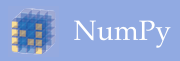
\includegraphics[scale=0.5]{imagenes/logos/numpy_logo.png}
\end{figure}
Biblioteca principal para cálculo científico con
\emph{Python}. Destaca por:
\begin{itemize}
\item Matrices N-dimensionales para albergar las imágenes.
\item Operaciones de álgebra lineal para las matrices.
\item Integración con el resto de bibliotecas del proyecto.
\end{itemize}

\subsection{matplotlib}
\begin{figure}[H]
  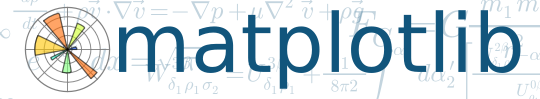
\includegraphics[scale=0.2]{imagenes/logos/matplotlib_logo.png}
\end{figure}
Biblioteca para dibujar gráficas en 2D y 3D en \emph{Python}. Muy
usada en el campo de visión computerizada para la visualización de
histogramas.

\subsection{OpenCV}
\begin{figure}[H]
  \hspace*{1.4cm}
  
\includegraphics[scale=0.2]{imagenes/logos/opencv_logo.png}
\end{figure}
Biblioteca de visión computerizada escrita en C++ y diseñada para
permitir su utilización en aplicaciones de tiempo real. Proporciona:
\begin{itemize}
\item Integración precisa con \emph{Python} y \emph{NumPy}.
\item Contiene funciones y algoritmos aplicables a todas las áreas de
  visión computerizada, especialmente para imágenes en 2D.
\item Creación de interfaces gráficas con paneles para facilitar la
  interacción con las técnicas aplicadas a las imágenes.
\end{itemize}

\subsection{SimpleCV}
\begin{figure}[H]
  \hspace*{1.7cm}
  
\includegraphics[scale=0.3]{imagenes/logos/simplecv_logo.png}
\end{figure}
Biblioteca de visión computerizada escrita en \emph{Python} sobre
\emph{OpenCV} que provee varios algoritmos complejos con una interfaz
mucho más simple que OpenCV\@.

\section{Bibliotecas propias}

Bibliotecas desarrolladas por y para el proyecto. Son envolturas a
otras bibliotecas con el objetivo de adaptarlas a las necesidades
surgidas con las \gls{tcoa}.

\subsection{Envoltura del módulo argparse}
Biblioteca escrita para facilitar la integración con el módulo
\emph{argparse} de la biblioteca estándar de \emph{Python} e
incorporar procesamiento de argumentos por consola como:
\begin{itemize}
\item Modo depuración.
\item Procesamiento de imágenes individuales.
\item Procesamiento de carpetas de imágenes.
\end{itemize}

\subsection{Extracción de zonas de interés}
Biblioteca que se encarga de extraer la región que se va a estudiar de
una \gls{tcoa}.

\subsection{Corrección de la inclinación}
Biblioteca que corrige la inclinación de las \gls{tcoa}, poniéndolas
horizontales si no lo están.

\let\thefootnote\relax\footnote{Todos los logos de terceros mostrados
  en este capítulo pertenecen a sus respectivos autores y están
  protegidos por las leyes de derechos de autor}

\chapter{Técnicas de visión computarizada}
Aquí se detallan todas las técnicas aplicadas o descartadas a lo largo
de la investigación. Incluye ejemplos de las tomografías para poder
relacionar la técnica con el resultado visual.\\
Toda la información presente en este capítulo ha sido redactada acorde
a las siguientes fuentes:
\begin{description}
\item[Hypermedia image processing
  reference]~\emph{\citep*{fisher1996hypermedia}}
\item[Computer Vision: Algorithms and
  Applications]~\emph{\citep*{szeliski2010computer}}
\item[Learning OpenCV]~\emph{\citep*{opencv_book-bib}}
\item[Guide to medical image analysis: methods and
  algorithms]~\emph{\citep*{toennies2012guide}}
\item[Tutorial de OpenCV para
  Python]~\emph{\citep*{opencv_tutorial-bib}}
\item[API de OpenCV]~\emph{\citep*{opencv_api-bib}}
\end{description}

\section{Conocimientos previos necesarios}

\subsection{Histogramas}\label{tecnica:histogramas}
Un histograma~\emph{\citep*[Chapter 7. Histograms and
  Matching]{opencv_book-bib}} es un gráfico con la distribución de
color o intensidades de la imagen. Por simplificación, supondremos
siempre una imagen en escala de grises. Es tan importante su estudio
dentro de la visión computarizada que se podría definir informalmente
como el gráfico que contiene la naturaleza de la imagen.
\begin{description}
\item[Columnas:] representan intensidades. Cada columna tiene una
  altura que corresponde proporcionalmente a la cantidad de píxeles
  con dicho valor.
\item[Dimensiones:] parámetros o número de datos a mostrar en el
  histograma. En el caso de una escala de grises sólo hay una
  dimensión, la intensidad, que puede ser 1 si el píxel tiene dicha
  intensidad o 0 en caso contrario.
\item[Rango:] es el número de columnas. En escala de grises el rango
  es de 256 columnas desde 0 hasta 255.
\end{description}

\subsubsection{Cálculo}
Para realizar el cálculo de un histograma y por simplificación se usa
una biblioteca. Tanto \emph{Numpy} como \emph{OpenCV} son capaces de
realizar los cálculos necesarios pero por eficiencia se usa
\emph{OpenCV} mediante
\mintinline{python}{cv2.equalizeHist()}\footnote{\url{http://docs.opencv.org/modules/imgproc/doc/histograms.html\#cv2.equalizeHist}}.

\subsubsection{Dibujado}
El resultado de un histograma es una matriz de \emph{Numpy} por lo
que, para poder dibujarla, tiene que usarse \emph{Matplotlib} o
transformar la matriz en una imagen de \emph{OpenCV}. Lo más simple es
usar
\mintinline{python}{matplotlib.pyplot.hist()}\footnote{\url{http://matplotlib.org/1.4.3/api/pyplot_api.html\#matplotlib.pyplot.hist}}.

\begin{figure}[H]
  \caption{Original}
  \centering \setlength\fboxsep{0pt} \setlength\fboxrule{0.5pt}
  \fbox{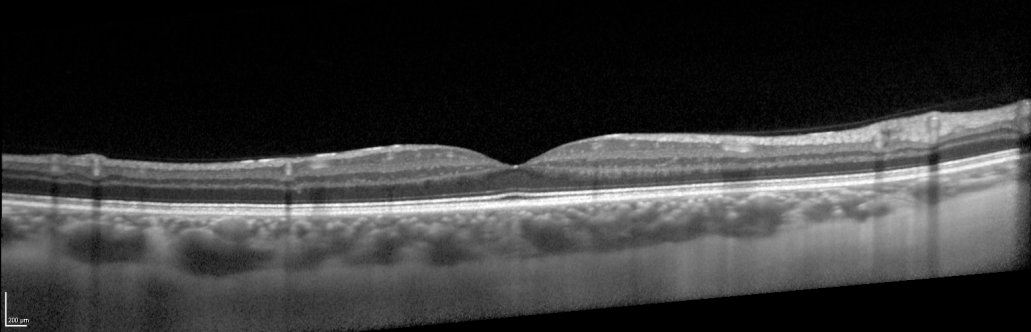
\includegraphics[width=\textwidth]{imagenes/tecnicas/histogramas/original_histogram.png}}
\end{figure}

\begin{figure}[H]
  \caption{Histograma}
  \centering \setlength\fboxsep{0pt} \setlength\fboxrule{0.5pt}
  \fbox{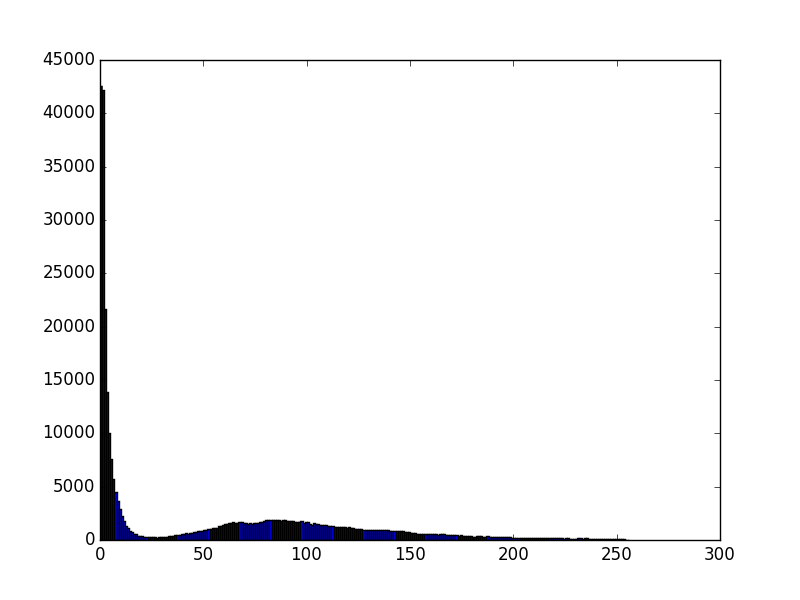
\includegraphics[scale=0.4]{imagenes/tecnicas/histogramas/histogram.png}}
\end{figure}

\subsubsection{Ecualización}
La ecualización~\emph{\citep*[3.1.4 Histogram
  equalization]{szeliski2010computer}} de un histograma consiste en
distribuir los píxeles por todo el rango. Esta acción aumenta el
contraste en aquellas imágenes que tienen la mayoría confinados en una
zona pequeña del rango.

\begin{figure}[H]
  \caption{Original}
  \centering \setlength\fboxsep{0pt} \setlength\fboxrule{0.5pt}
  \fbox{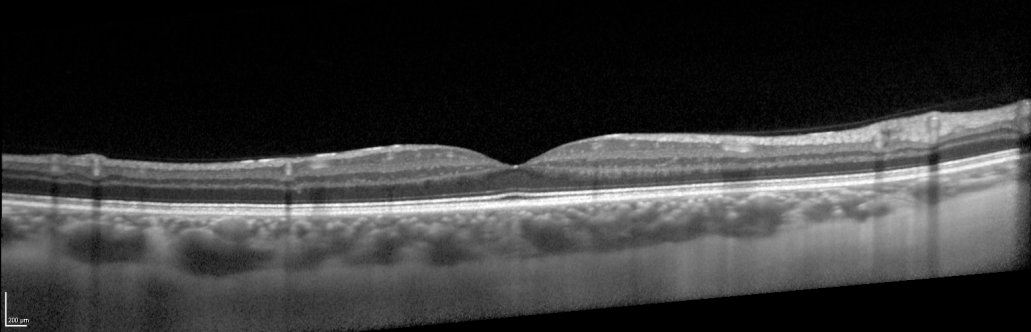
\includegraphics[width=\textwidth]{imagenes/tecnicas/histogramas/original_histogram.png}}
\end{figure}

\begin{figure}[H]
  \caption{Histograma ecualizado}
  \centering \setlength\fboxsep{0pt} \setlength\fboxrule{0.5pt}
  \fbox{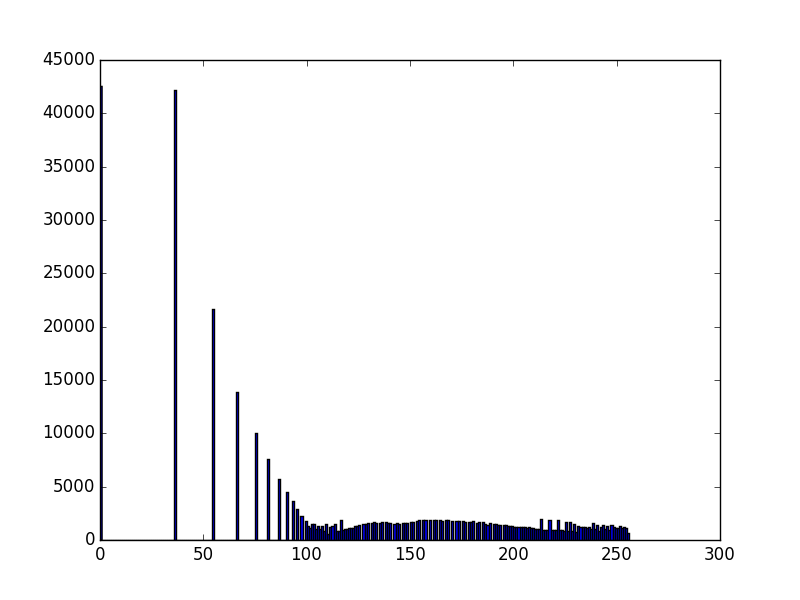
\includegraphics[scale=0.4]{imagenes/tecnicas/histogramas/equalization.png}}
\end{figure}

\begin{figure}[H]
  \caption{Original ecualizada}
  \centering \setlength\fboxsep{0pt} \setlength\fboxrule{0.5pt}
  \fbox{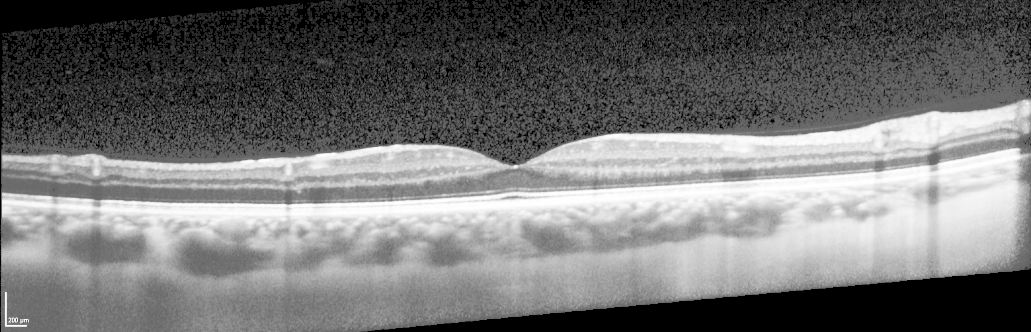
\includegraphics[width=\textwidth]{imagenes/tecnicas/histogramas/equalization_histogram.png}}
\end{figure}

Normalmente y como se puede apreciar, la aplicación de una
\emph{ecualización} a la imagen puede provoca que las zonas intensas
lo sean todavía más, lo que aumenta la luminosidad de la imagen. Para
evitar esto, se utilizan \emph{ecualizaciones adaptativas} más
conocidas por las siglas \emph{AHE} \emph{\citep*[Image enhancement
  techniques for cockpit displays]{ketcham1974image}} bastante
complejas tanto para mejorar el contraste de las zonas más intensas
como el posible ruido generado con técnicas de \emph{contraste
  limitado} (\emph{CLAHE}). Técnicas muy especialmente utilizadas en
imágenes médicas como demuestran las de ejemplo usadas en
\emph{\citep*[Adaptive histogram equalization and its
  variations]{pizer1987adaptive}}. \emph{OpenCV} proporciona
\mintinline{python}{cv2.createCLAHE()}\footnote{\url{https://opencv-python-tutroals.readthedocs.org/en/latest/py\_tutorials/py_imgproc/py\_histograms/py\_histogram_equalization/py\_histogram_equalization.html\#clahe-contrast-limited-adaptive-histogram-equalization}}.

\begin{figure}[H]
  \caption{Original}
  \centering \setlength\fboxsep{0pt} \setlength\fboxrule{0.5pt}
  \fbox{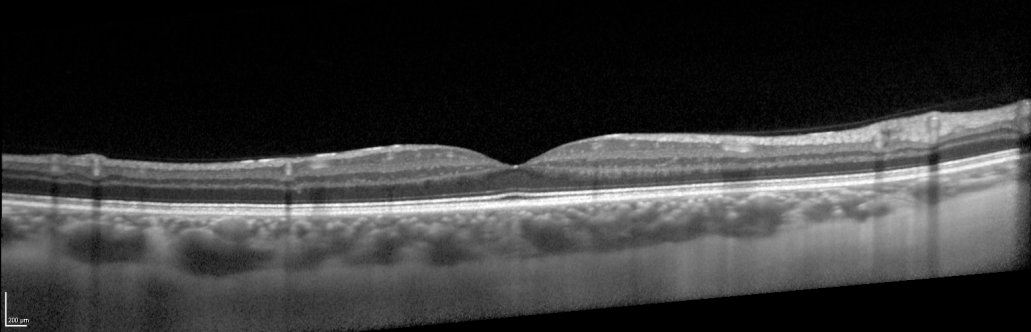
\includegraphics[width=\textwidth]{imagenes/tecnicas/histogramas/original_histogram.png}}
\end{figure}

\begin{figure}[H]
  \caption{Histograma ecualizado con CLAHE}
  \centering \setlength\fboxsep{0pt} \setlength\fboxrule{0.5pt}
  \fbox{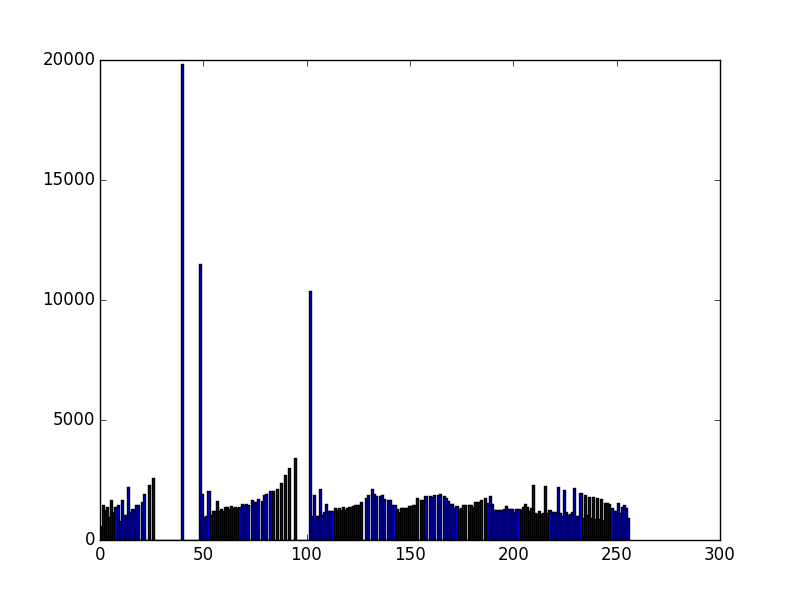
\includegraphics[scale=0.4]{imagenes/tecnicas/histogramas/clahe_equalization.png}}
\end{figure}

\begin{figure}[H]
  \caption{Original ecualizada con CLAHE}
  \centering \setlength\fboxsep{0pt} \setlength\fboxrule{0.5pt}
  \fbox{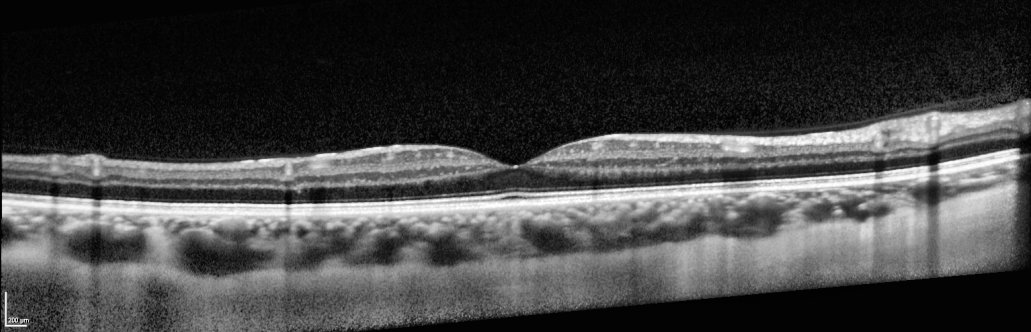
\includegraphics[width=\textwidth]{imagenes/tecnicas/histogramas/clahe.png}}
\end{figure}


\subsection{Convolución de matrices}
La \emph{convolución}\emph{~\citep*[3.2 Linear
  filtering]{szeliski2010computer}}\emph{~\citep*[A.6
  Convolution]{fisher1996hypermedia}} de una matriz sobre una imagen,
que al fin y al cabo es otra matriz, es la principal base de la
mayoría de las técnicas aquí descritas. \\
Un \emph{kernel} es una matriz fija de coeficientes numéricos y
dimensión \textbf{impar} que se usa en todas las técnicas de este
capítulo para tener un elemento como el elemento central. \\
Para calcular la convolución de un píxel concreto se sitúa éste en el
centro del \emph{kernel} y se calcula su valor con respecto a los
píxeles de alrededor, multiplicando su valor por el valor del
\emph{kernel} para esa posición. Finalmente, cada multiplicación se
suma y se guarda el resultado total en la posición central. Este
proceso se repite con cada píxel. \\
La ecuación que representa el proceso anterior, definiendo la imagen
como $I(x, y)$, el \emph{kernel} como $K(i, j)$ (donde
$0 < i < M_j - 1$ y $0 < j < M_j - 1$) y el centro de la matriz de
convolución es $(c_i, c_j)$ definimos la imagen resultante como
\begin{equation*}
  R(x, y) = \sum_{i=0}^{M_i-1} \sum_{j=0}^{M_j-1}  I(x + i - c_i, y + j - c_j)K(i,j)
\end{equation*}
En el caso de \emph{OpenCV}, tanto la imagen original \emph{I} como la
imagen resultante \emph{R} son del mismo tamaño. Esto se debe a que
\emph{OpenCV} duplica el borde de manera virtual para que el
\emph{kernel} de convolución se pueda aplicar hasta el mismo borde de
la imagen. Hay distintas maneras de duplicar el borde pero aquí sólo
se muestra la más simple y sobre el eje de abscisas:
\begin{center}
  $imagen(-dx, y) = imagen(0, y)$
  \\
  $imagen(w + dx) = imagen(w - 1, y)$
\end{center}


\section{Operaciones básicas}
\subsection{Acceso a píxeles}
El acceso a los píxeles de una imagen se realiza a través de
\emph{Numpy} como una matriz de dimensiones $y \times x$, siendo $y$
la altura y $x$ el ancho.
\begin{minted}{Python}
  pixel = imagen[y, x]
\end{minted}

\subsection{Propiedades}
Las dos propiedades más utilizadas de las imágenes son su altura y
anchura.  Se pueden obtener con la función \emph{shape}.
\begin{minted}{Python}
  y, x = imagen.shape
\end{minted}

\subsection{Región de interés}\label{tecnica:roi}
La región de interés (ROI) de una imagen es la zona que estamos
interesados en procesar. Se expresa mediante los vértices opuestos de
un rectángulo o cuadrado definidos con el par de píxeles
$\left(y_1,x_1\right)\left(y_2,x_2\right)$ de la imagen
\begin{minted}{Python}
  roi = imagen[y1:y2, x1:x2]
\end{minted}

\section{Operaciones aritméticas}
\subsection{Superposición}
La superposición\emph{~\citep[3.1.1 Pixel transforms, 3.1.3
  Compositing and matting]{szeliski2010computer}} de dos imágenes (del
mismo tipo, profundidad o una que sea un valor escalar) es la suma
matricial de sus píxeles, asignando a cada imagen un peso diferente
para dar la sensación de superposición y transparencia. La función
sería:
\begin{equation*}
  g(n) = (1 - \alpha)f_0(n) + \alpha f_1(n)
\end{equation*}
Donde \emph{n} representa un punto de la imagen, \emph{$\alpha$} es una
constante entre $0$ y $1$, y \emph{$f_0$} y \emph{$f_1$} las imágenes.
Expresado en forma de coordenadas:
\begin{equation*}
  g(x, y) = (1 - \alpha)f_0(x, y) + \alpha f_1(x, y)
\end{equation*}
$x$ e $y$ representan las coordenadas (horizontal y vertical
respectivamente). \emph{OpenCV} proporciona para realizar esta técnica
\mintinline{python}{cv2.addWeighted}\footnote{\url{http://docs.opencv.org/modules/core/doc/operations_on_arrays.html\#cv2.addWeighted}}


\section{Cambio de espacio de color}\label{tecnica:cambio-color}
Un espacio de color~\emph{\citep*[Changing
  Colorspaces]{opencv_tutorial-bib}} es un modelo matemático abstracto
que describe la forma en la que los colores pueden representarse como
tuplas de
números. \emph{RGB}, \emph{HSV} o escala de grises son ejemplos de espacios de color. \\
El espacio de color de una imagen se puede cambiar con
\mintinline{python}{cv2.cvtColor()}\footnote{\url{http://docs.opencv.org/modules/imgproc/doc/miscellaneous\_transformations.html\#cv2.cvtColor}}. Esta
que permite las siguientes conversiones en las dos direcciones:
\begin{itemize}
\item \textbf{RGB} --- \textbf{escala de grises}.
\item \textbf{RGB} --- \textbf{CIE XYZ}.
\item \textbf{RGB} --- \textbf{YCrCb JPEG} (o YCC).
\item \textbf{RGB} --- \textbf{HSV}.
\item \textbf{RGB} --- \textbf{HLS}.
\item \textbf{RGB} --- \textbf{Bayer}.
\end{itemize}
Estas transformaciones permiten la detección rápida y sencilla de
características de interés. \\
Para este proyecto se han usado las que implican \emph{RGB} y escala
de grises porque a pesar de la elección de generar con la máquina las
\gls{tco} en escala de grises, realmente las almacena como \emph{RGB}.

\section{Operaciones de \emph{threshold}}
Las operaciones de \emph{threshold}~\emph{\citep*[Image
  Thresholding]{opencv_tutorial-bib}}~\emph{\citep*[Threshold]{opencv_book-bib}}~\emph{\citep*[6.5
  Thresholding]{toennies2012guide}} convierten los píxeles de una
imagen (en escala de grises $\left[0 \dots 255\right]$) superiores a
un valor, conocido como valor de umbral, a blanco $255$ o a negro $0$,
según el \emph{threshold} aplicado. Para aplicarlos, se utiliza
\mintinline{python}{cv2.threshold()}\footnote{\url{http://docs.opencv.org/modules/imgproc/doc/miscellaneous_transformations.html\#cv2.threshold}}.
\subsection{Simples}
\subsubsection{cv2.THRESH\_BINARY o
  \emph{Binarización}}\label{tecnica:threshold-binario}
Todos los píxeles con un valor mayor que el valor de umbral se
transforman, asignándoles el valor máximo. Los que no lo superen,
adquieren el valor mínimo.  La expresión es
\begin{equation*}
  destino(x, y) =
  \begin{cases}
    255 & \text{si } entrada(x, y) > umbral \\
    0 & \text{cualquier otro caso}
  \end{cases}
\end{equation*}
Ejemplo para un valor de umbral de $127$ (Arriba original y abajo el
resultado obtenido tras aplicar el filtro):

\begin{figure}[H]
  \caption{Original}
  \centering \setlength\fboxsep{0pt} \setlength\fboxrule{0.5pt}
  \fbox{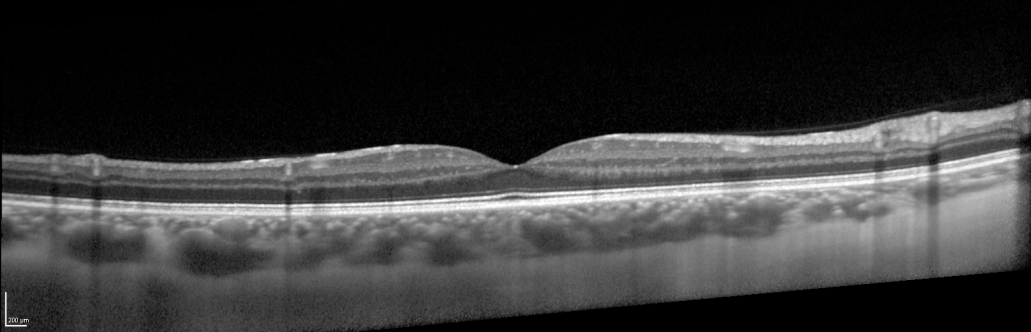
\includegraphics[width=\textwidth]{imagenes/tecnicas/EjemploTecnicasThresholdOriginal.png}}
\end{figure}

\begin{figure}[H]
  \centering \setlength\fboxsep{0pt} \setlength\fboxrule{0.5pt}
  \fbox{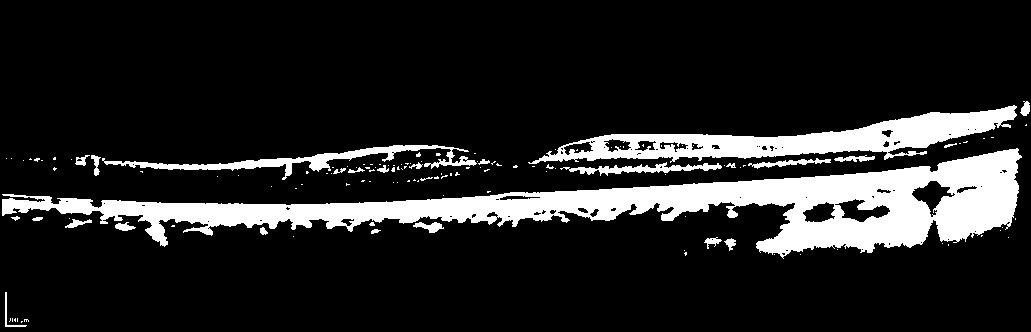
\includegraphics[width=\textwidth]{imagenes/tecnicas/EjemploTecnicasThresholdBinary_127.png}}
  \caption{Treshold Binario}
\end{figure}

\subsubsection{cv2.THRESH\_BINARY\_INV o \emph{Binarización inversa}}
Es la operación contraria al anterior: a los píxeles con un valor
mayor que el valor de umbral se les asigna el valor mínimo, mientras
que los demás adquieren el valor máximo. La expresión es
\begin{equation*}
  destino(x, y) =
  \begin{cases}
    0 & \text{si } entrada(x, y) > umbral \\
    255 & \text{cualquier otro caso}
  \end{cases}
\end{equation*}
Ejemplo para un valor de umbral de $127$ (Arriba original y abajo el
resultado obtenido tras aplicar el filtro):

\begin{figure}[H]
  \caption{Original}
  \centering \setlength\fboxsep{0pt} \setlength\fboxrule{0.5pt}
  \fbox{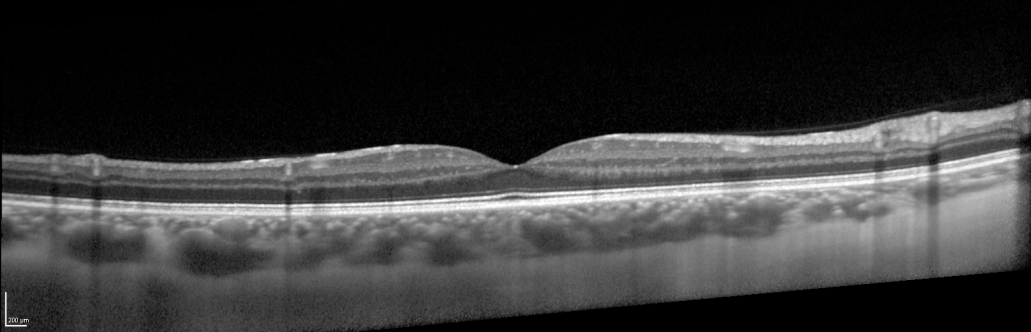
\includegraphics[width=\textwidth]{imagenes/tecnicas/EjemploTecnicasThresholdOriginal.png}}
\end{figure}

\begin{figure}[H]
  \centering \setlength\fboxsep{0pt} \setlength\fboxrule{0.5pt}
  \fbox{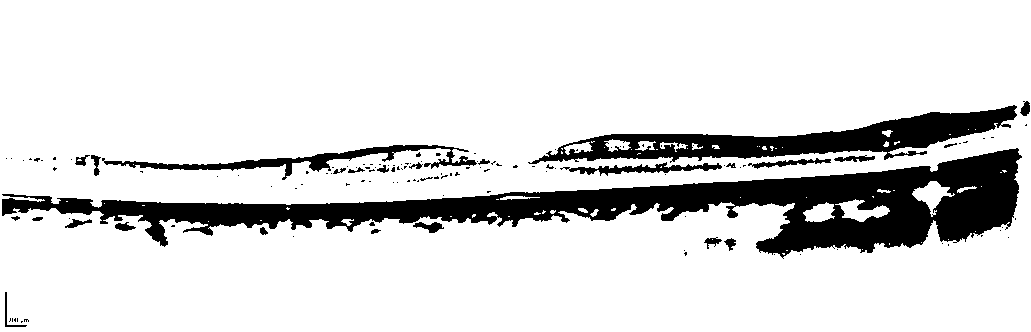
\includegraphics[width=\textwidth]{imagenes/tecnicas/EjemploTecnicasThresholdBinaryInv_127.png}}
  \caption{Threshold Binario Inverso}
\end{figure}


\subsubsection{cv2.THRESH\_TRUNC o \emph{Truncamiento}}
Se trunca el valor de los píxeles de forma que todos los píxeles que
superen el valor de umbral toman dicho valor. En caso contrario se
conserva el valor original. La expresión es
\begin{equation*}
  destino(x, y) =
  \begin{cases}
    umbral & \text{si } entrada(x, y) > umbral \\
    entrada(x, y) & \text{cualquier otro caso}
  \end{cases}
\end{equation*}
Ejemplo para un valor de umbral de $127$ (Arriba original y abajo el
resultado obtenido tras aplicar el filtro):

\begin{figure}[H]
  \caption{Original}
  \centering \setlength\fboxsep{0pt} \setlength\fboxrule{0.5pt}
  \fbox{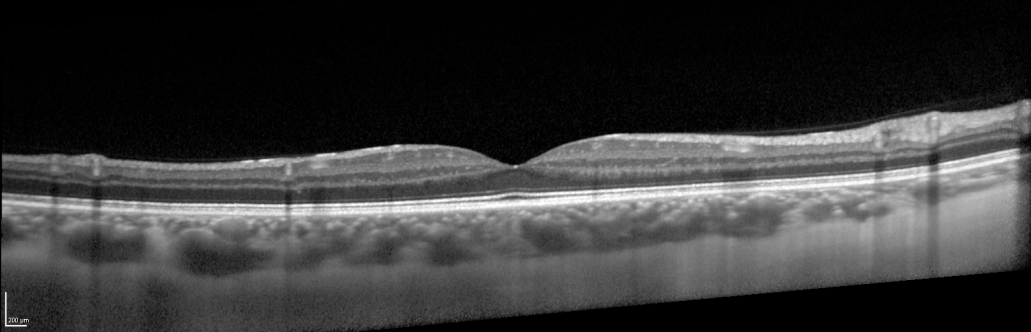
\includegraphics[width=\textwidth]{imagenes/tecnicas/EjemploTecnicasThresholdOriginal.png}}
\end{figure}

\begin{figure}[H]
  \centering \setlength\fboxsep{0pt} \setlength\fboxrule{0.5pt}
  \fbox{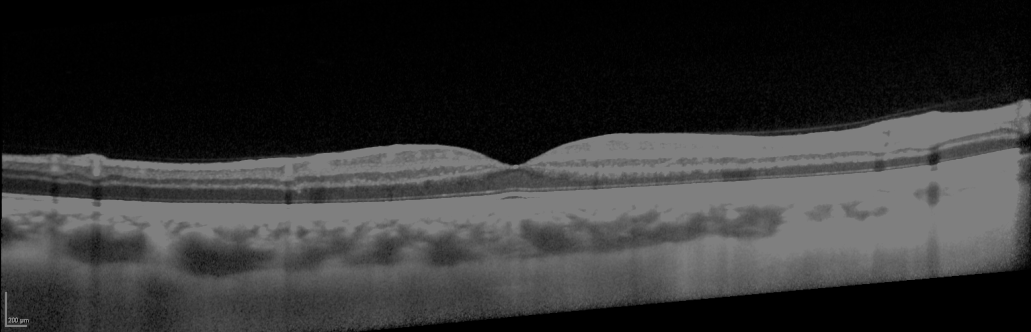
\includegraphics[width=\textwidth]{imagenes/tecnicas/EjemploTecnicasThresholdTrunc_127.png}}
  \caption{Threshold de Truncado}
\end{figure}


\subsubsection{cv2.THRESH\_TOZERO}
Es la operación contraria a la anterior: los píxeles que superen el
valor del umbral conservan su valor original, mientras que en el caso
contrario se les aplica el valor mínimo. La expresión es
\begin{equation*}
  destino(x, y) =
  \begin{cases}
    entrada(x, y) & \text{si } entrada(x, y) > umbral \\
    0 & \text{cualquier otro caso}
  \end{cases}
\end{equation*}
Ejemplo para un valor de umbral de $127$ (Arriba original y abajo el
resultado obtenido tras aplicar el filtro):

\begin{figure}[H]
  \caption{Original}
  \centering \setlength\fboxsep{0pt} \setlength\fboxrule{0.5pt}
  \fbox{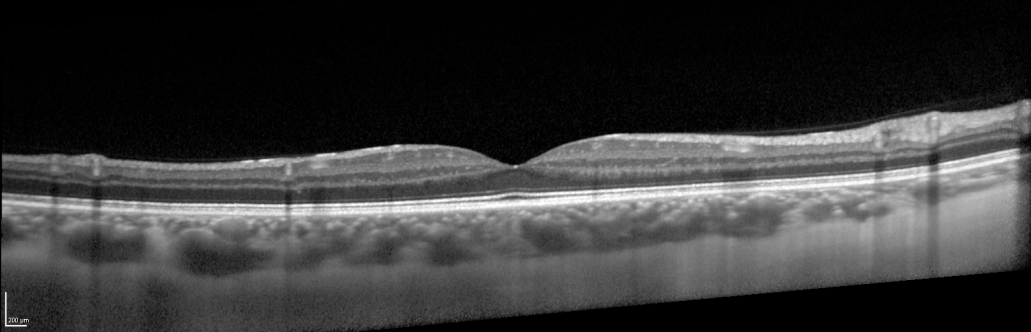
\includegraphics[width=\textwidth]{imagenes/tecnicas/EjemploTecnicasThresholdOriginal.png}}
\end{figure}

\begin{figure}[H]
  \centering \setlength\fboxsep{0pt} \setlength\fboxrule{0.5pt}
  \fbox{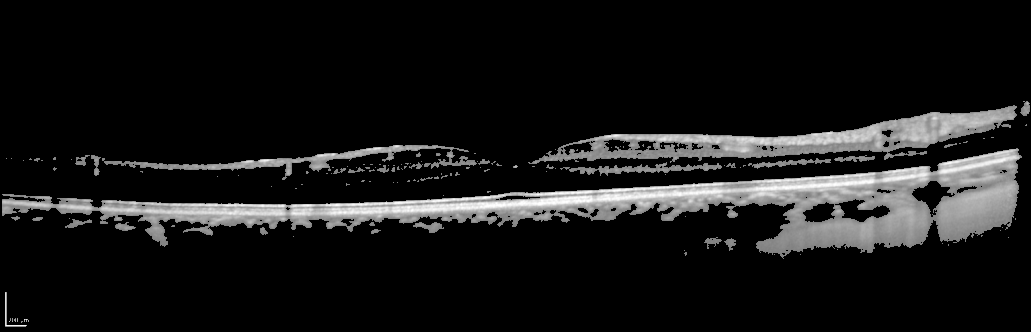
\includegraphics[width=\textwidth]{imagenes/tecnicas/EjemploTecnicasThresholdTo0_127.png}}
  \caption{Threshold to Zero}
\end{figure}

\subsubsection{cv2.THRESH\_TOZERO\_INV}
A los píxeles que superen el valor de umbral se les aplica el valor
mínimo, mientras que en caso contrario conservan el valor original. La
expresión es
\begin{equation*}
  destino(x, y) =
  \begin{cases}
    0  & \text{si } entrada(x, y) > umbral \\
    entrada(x, y) & \text{cualquier otro caso}
  \end{cases}
\end{equation*}
Ejemplo para un valor de umbral de $127$ (Arriba original y abajo el
resultado obtenido tras aplicar el filtro):

\begin{figure}[H]
  \caption{Original}
  \centering \setlength\fboxsep{0pt} \setlength\fboxrule{0.5pt}
  \fbox{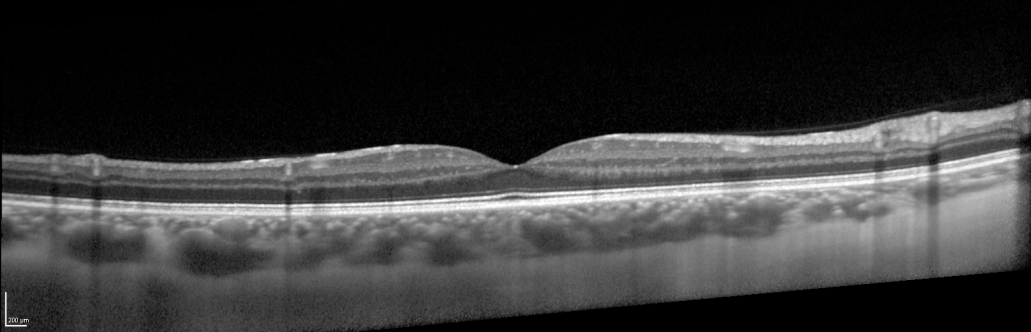
\includegraphics[width=\textwidth]{imagenes/tecnicas/EjemploTecnicasThresholdOriginal.png}}
\end{figure}

\begin{figure}[H]
  \centering \setlength\fboxsep{0pt} \setlength\fboxrule{0.5pt}
  \fbox{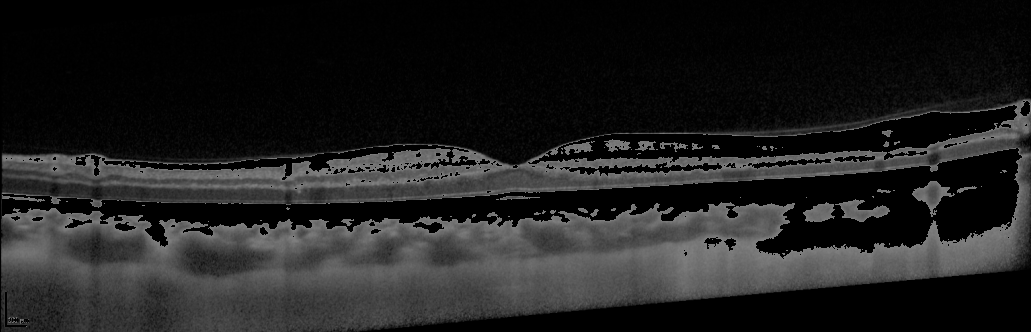
\includegraphics[width=\textwidth]{imagenes/tecnicas/EjemploTecnicasThresholdTo0Inv_127.png}}
  \caption{Threshold to Zero Inverso}
\end{figure}

\subsection{Adaptativos}
En imágenes uniformes aplicar valores umbral globales y fijos suele
ser una buena opción pero para imágenes no uniformes hay que adaptar
dicho valor a cada área de la imagen. Por ello, se aplican las
técnicas siguientes. En ambas, el área a realizar el
\emph{threshold}~\emph{\citep*[6.2 Adaptive
  Thresholding]{fisher1996hypermedia}} depende del tamaño del
\emph{kernel} usado mediante
\mintinline{python}{cv2.adaptiveThreshold()}\footnote{\url{http://docs.opencv.org/modules/imgproc/doc/miscellaneous\_transformations.html\#cv2.adaptiveThreshold}}.

\subsubsection{cv2.ADAPTIVE\_THRESH\_MEAN\_C}
El valor de cada píxel se establece por la media de sus vecinos
restándole una constante $C$.

\begin{figure}[H]
  \caption{Original}
  \centering \setlength\fboxsep{0pt} \setlength\fboxrule{0.5pt}
  \fbox{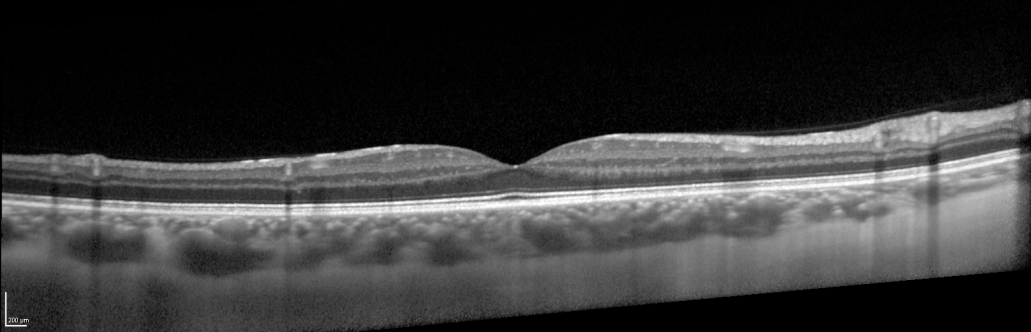
\includegraphics[width=\textwidth]{imagenes/tecnicas/EjemploTecnicasThresholdOriginal.png}}
\end{figure}

\begin{figure}[H]
  \centering \setlength\fboxsep{0pt} \setlength\fboxrule{0.5pt}
  \fbox{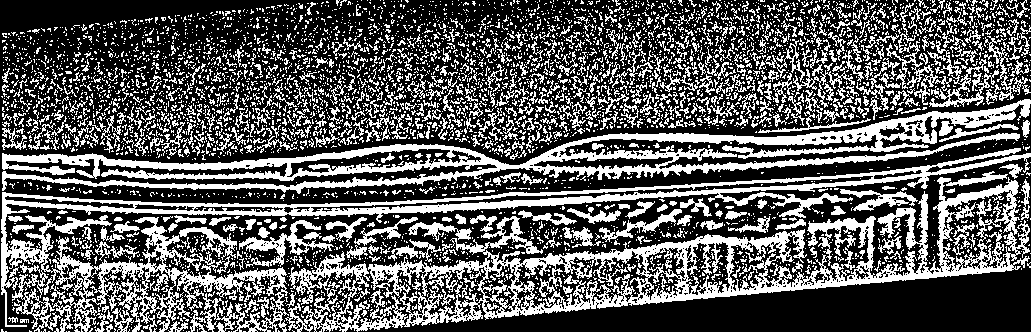
\includegraphics[width=\textwidth]{imagenes/tecnicas/EjemploTecnicasThresholdAdaptiveMeanKernel11Constant2.png}}
  \caption{Mean Adaptive Threshold}
\end{figure}

\subsubsection{cv2.ADAPTIVE\_THRESH\_GAUSSIAN\_C}\label{tecnica:threshold-adaptativo-gauss}
El valor de cada píxel se establece por el resultado de una función
Gaussiana a partir de sus vecinos y restándole una constante $C$.

\begin{figure}[H]
  \caption{Original}
  \centering \setlength\fboxsep{0pt} \setlength\fboxrule{0.5pt}
  \fbox{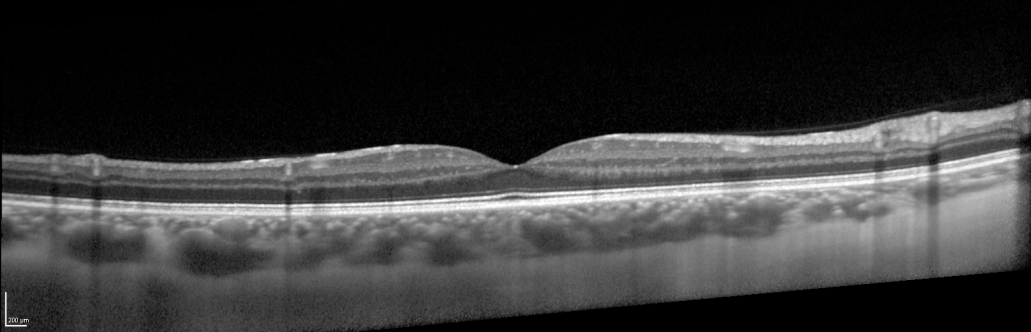
\includegraphics[width=\textwidth]{imagenes/tecnicas/EjemploTecnicasThresholdOriginal.png}}
\end{figure}

\begin{figure}[H]
  \centering \setlength\fboxsep{0pt} \setlength\fboxrule{0.5pt}
  \fbox{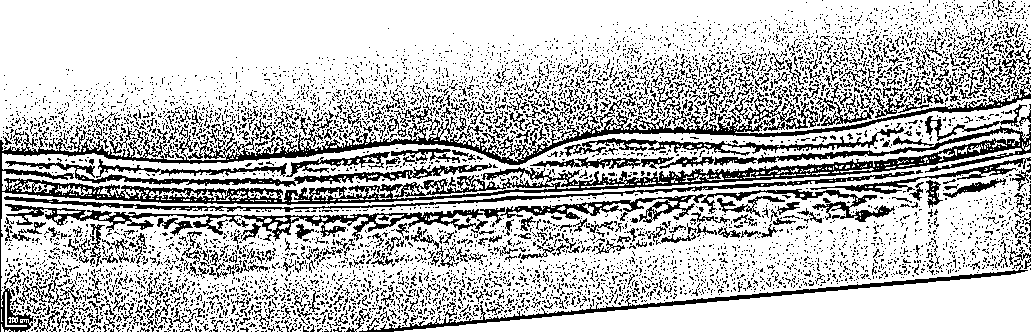
\includegraphics[width=\textwidth]{imagenes/tecnicas/EjemploTecnicasThresholdAdaptiveGaussianKernel11Constant2.png}}
  \caption{Gaussian Adaptive Threshold}
\end{figure}

\subsection{Otsu}\label{tecnica:threshold-otsu}
Este \emph{threshold}\emph{~\citep*[A threshold selection method from
  gray-level histograms]{otsu1975threshold}} calcula el valor umbral a
partir del histograma de la imagen. La precisión de esta técnica
depende de que el histograma sea lo más bimodal posible, en los que
predomina dos columnas. Para ello, se utiliza
\mintinline{python}{cv2.threshold()}\footnote{\url{http://docs.opencv.org/modules/imgproc/doc/miscellaneous\_transformations.html\#cv2.threshold}}.

\begin{figure}[H]
  \caption{Original}
  \centering \setlength\fboxsep{0pt} \setlength\fboxrule{0.5pt}
  \fbox{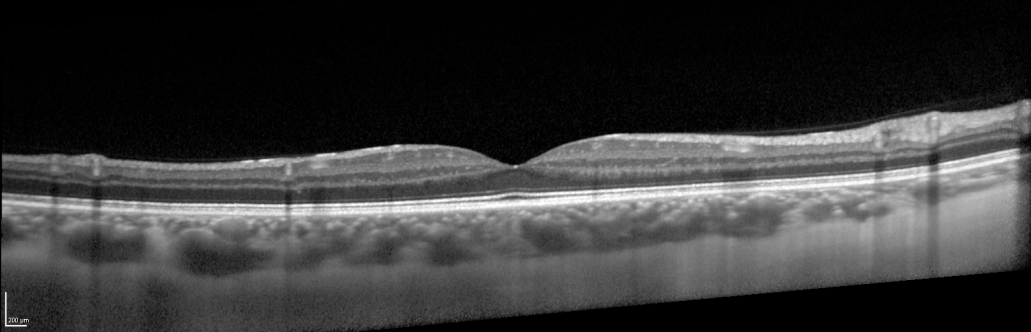
\includegraphics[width=\textwidth]{imagenes/tecnicas/EjemploTecnicasThresholdOriginal.png}}
\end{figure}

\begin{figure}[H]
  \centering \setlength\fboxsep{0pt} \setlength\fboxrule{0.5pt}
  \fbox{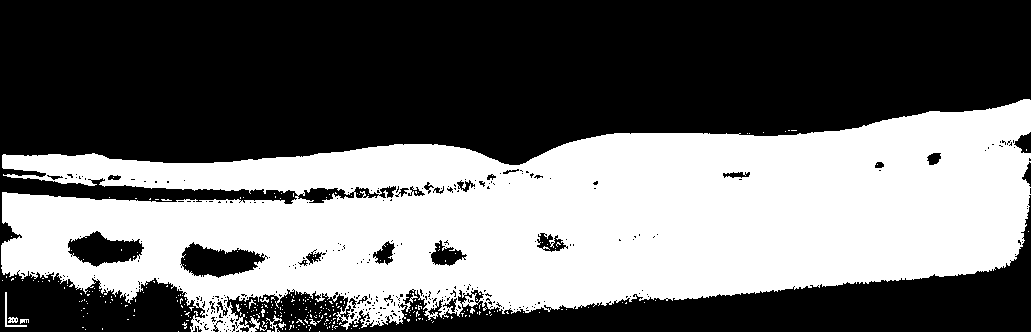
\includegraphics[width=\textwidth]{imagenes/tecnicas/EjemploTecnicasThresholdOtsu.png}}
  \caption{Otsu Threshold}
\end{figure}

\section{Transformaciones geométricas}
Las transformaciones geométricas~\emph{\citep*[Stretch, Shrink, Warp,
  and Rotate]{opencv_book-bib}} son aquellas técnicas en las que se
aplica una matriz o \emph{kernel} de transformación a la imagen
original.
\subsection{Rotación}
Para rotar una imagen desde un ángulo $\theta$ se opera con la siguiente
matriz de transformación.
\begin{equation*}
  M =
  \begin{bmatrix}
    \cos \theta & -\sin \theta \\ \sin \theta & \cos \theta
  \end{bmatrix}
\end{equation*}
\emph{OpenCV} además, facilita una matriz de rotación escalable con
centro ajustable para el punto que se prefiera.
\begin{equation*}
  \begin{bmatrix}
    \alpha & \beta & (1 - \alpha) \cdot centro_x - \beta \cdot centro_y \\
    - \beta & \alpha & \beta \cdot centro_x + (1 - \alpha) \cdot centro_y
  \end{bmatrix}
\end{equation*}
donde:
\begin{center}
  $ \alpha = escala \cdot \cos \theta $
  \\
  $ \beta = escala \cdot \sin \theta $
\end{center}
Para facilitar todavía más la rotación, \emph{OpenCV} proporciona
\mintinline{python}{cv2.getRotationMatrix2D()}\footnote{\url{http://docs.opencv.org/modules/imgproc/doc/geometric\_transformations.html\#cv2.getRotationMatrix2D}}
para posteriormente aplicar la afinidad con
\mintinline{python}{cv2.warpAffine()}\footnote{\url{http://docs.opencv.org/modules/imgproc/doc/geometric\_transformations.html\#cv2.warpAffine}}.\\

Ejemplo de rotación de $-5º$ de una imagen. \emph{OpenCV} tiene el eje
de coordenadas en la parte superior izquierda con respecto a su
centro. A continuación se muestra una imagen ilustrativa extraída
de~\citep*{opencv_tutorial-bib}~\footnote{Derecho de
  cita e ilustración de la enseñanza\\
  \url{http://www.riate.org/version/v1/recursos/cursolicenciasnavegable/derecho_de_cita_e_ilustracin_de_la_enseanza.html}\\
  \url{http://www.boe.es/boe/dias/2006/07/08/pdfs/A25561-25572.pdf}}.

\begin{figure}[H]
  \caption{Eje de coordenadas en \emph{OpenCV}}
  \centering \setlength\fboxsep{0pt} \setlength\fboxrule{0.5pt}
  \fbox{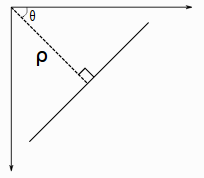
\includegraphics[scale=0.5]{imagenes/tecnicas/houghReference.png}}
\end{figure}

\begin{figure}[H]
  \caption{Original}
  \centering \setlength\fboxsep{0pt} \setlength\fboxrule{0.5pt}
  \fbox{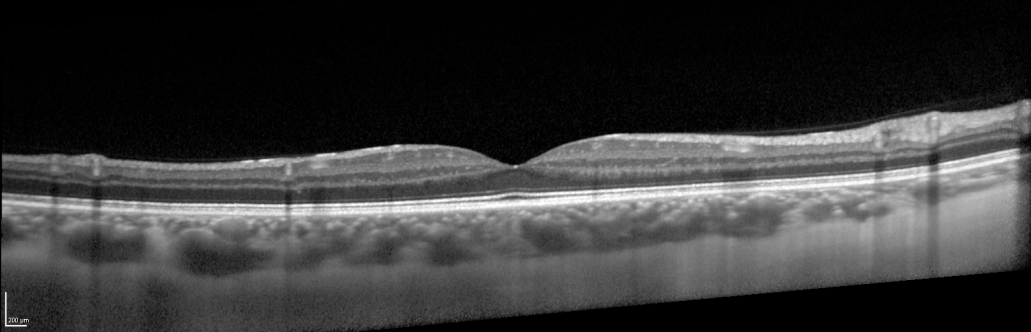
\includegraphics[width=\textwidth]{imagenes/tecnicas/EjemploTecnicasThresholdOriginal.png}}
\end{figure}

\begin{figure}[H]
  \centering \setlength\fboxsep{0pt} \setlength\fboxrule{0.5pt}
  \fbox{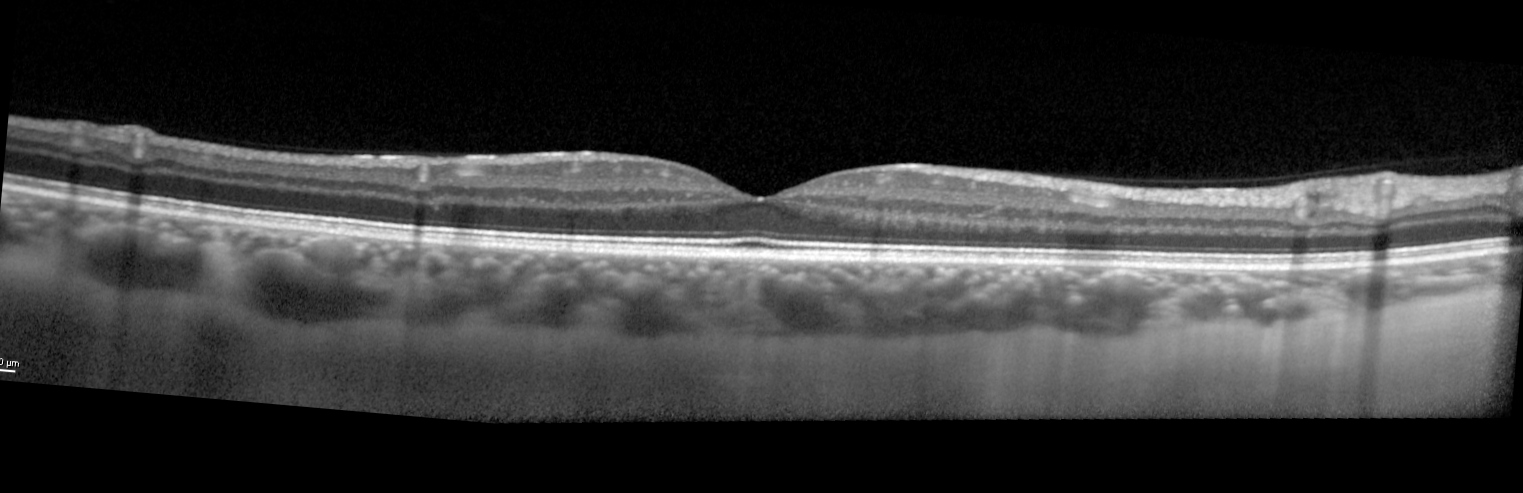
\includegraphics[width=\textwidth]{imagenes/tecnicas/EjemploTecnicasHorizontal-5.png}}
  \caption{Rotada}
\end{figure}

\section{\emph{Blur}}
\emph{Blur}~\emph{\citep*[Smoothing]{opencv_book-bib}}~\emph{\citep*[3.3.1
  Non-linear filtering]{szeliski2010computer}}~\emph{\citep*[4.3 Noise
  Reduction]{toennies2012guide}} o suavizado es una técnica usada con
el objetivo principal de reducir el ruido y los artefactos (contenido
de alta frecuencia) de la imagen, aunque también se usa para disminuir
la resolución. Se basa en aplicar a la imagen un \emph{kernel} de
convolución.
\subsection{Basado en la media}
En el caso de un \emph{blur}, se suman todos los valores de los
píxeles contenidos en la matriz y se divide entre el número de
vecinos. El \emph{kernel} a aplicar es el siguiente
\begin{equation*}
  K = \frac{1}{n}
  \begin{bmatrix}
    1_{11} & 1_{12} & \cdots & 1_{1n} \\
    1_{21} & 1_{22} & \cdots & 1_{2n} \\
    \vdots & \vdots & \ddots & \vdots \\
    1_{n1} & 1_{n2} & \cdots & 1_{nn} \\
  \end{bmatrix}
  \text{siendo \emph{n} un número impar}
\end{equation*}

A modo de ejemplo, el \emph{kernel} de dimensión $3\times3$ es
\begin{equation*}
  K = \frac{1}{9}
  \begin{bmatrix}
    1 & 1 & 1 \\
    1 & 1 & 1 \\
    1 & 1 & 1 \\
  \end{bmatrix}
\end{equation*}

Y a continuación y para mayor énfasis, la aplicación de un
\emph{kernel} de tamaño $7 \times 7$. Para ello, se utiliza
\mintinline{python}{cv2.blur()}\footnote{\url{http://docs.opencv.org/modules/imgproc/doc/filtering.html\#cv2.blur}}.\\


\begin{figure}[H]
  \caption{Original}
  \centering \setlength\fboxsep{0pt} \setlength\fboxrule{0.5pt}
  \fbox{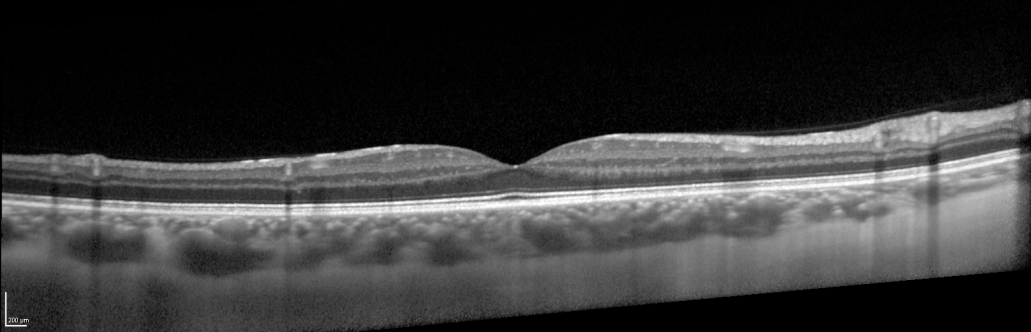
\includegraphics[width=\textwidth]{imagenes/tecnicas/EjemploTecnicasThresholdOriginal.png}}
\end{figure}

\begin{figure}[H]
  \centering \setlength\fboxsep{0pt} \setlength\fboxrule{0.5pt}
  \fbox{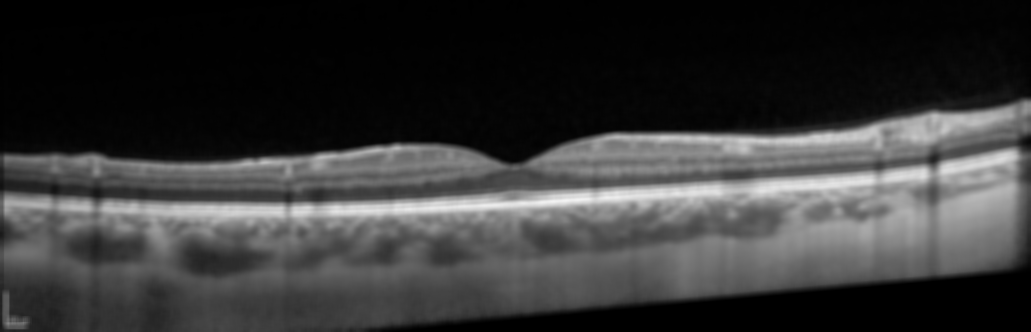
\includegraphics[width=\textwidth]{imagenes/tecnicas/EjemploTecnicasBlur7.png}}
  \caption{Blur}
\end{figure}

\subsection{Basado en una función Gaussiana}
Esta técnica es la que mejor resultados suele dar, especialmente si se
utiliza para reducir el ruido generado por un \emph{kernel
  Gaussiano}. Cabe destacar que al aplicar este método puede dar como
resultado valores de píxeles que no estuvieran en la imagen
original. Este \emph{Blur} es el menos eficiente de todos pero
\emph{OpenCV} mediante
\mintinline{python}{cv2.GaussianBlur()}\footnote{\url{http://docs.opencv.org/modules/imgproc/doc/filtering.html\#cv2.GaussianBlur}}
lo optimiza para las sigmas $\sigma_x$ y $\sigma_y$ predeterminadas de
los \emph{kernels} de $3\times3$, $5\times5$ y $7\times7$. Debido a
esto, sólo mostraremos como se
generan estas sigmas predeterminas y un ejemplo con ellas.\\
\emph{OpenCV} obliga a introducir $\sigma_x$ y en el caso de que este sea
$0$, se determinan ambos sigmas a partir del tamaño del \emph{kernel}
introducido mediante las fórmulas siguientes:
\begin{equation*}
  \hspace{0.25cm}\sigma_x = \left(\frac{n_x}{2} - 1 \right) \cdot 0,30 + 0,80 \hspace{0.5cm} n_x = \text{anchura del \emph{kernel}}
\end{equation*}
\begin{equation*}
  \sigma_y = \left(\frac{n_y}{2} - 1 \right) \cdot 0,30 + 0,80 \hspace{0.5cm} n_y = \text{altura del \emph{kernel}}
\end{equation*}
Y la función \emph{Gaussiana} en la que se aplican:
\begin{equation*}
  Gaussiana(x, y) = \frac{1}{\sqrt{2 \pi \sigma^{2}}}e^{- \frac{x^{2}+y^{2}}{2\sigma^{2}}}
\end{equation*}
En el siguiente ejemplo se aplica un \emph{Blur} con basado en una función
Gaussiana con \emph{kernel} de $23 \times 23$, a partir del cual se
calculan las \emph{sigmas}:

\begin{figure}[H]
  \caption{Original}
  \centering \setlength\fboxsep{0pt} \setlength\fboxrule{0.5pt}
  \fbox{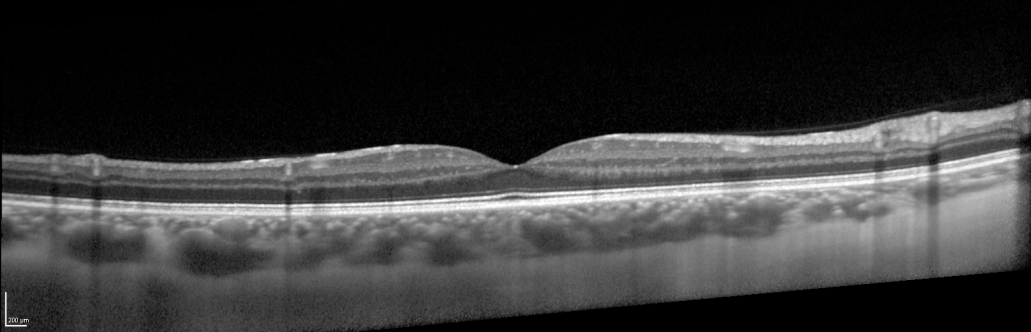
\includegraphics[width=\textwidth]{imagenes/tecnicas/EjemploTecnicasThresholdOriginal.png}}
\end{figure}

\begin{figure}[H]
  \centering \setlength\fboxsep{0pt} \setlength\fboxrule{0.5pt}
  \fbox{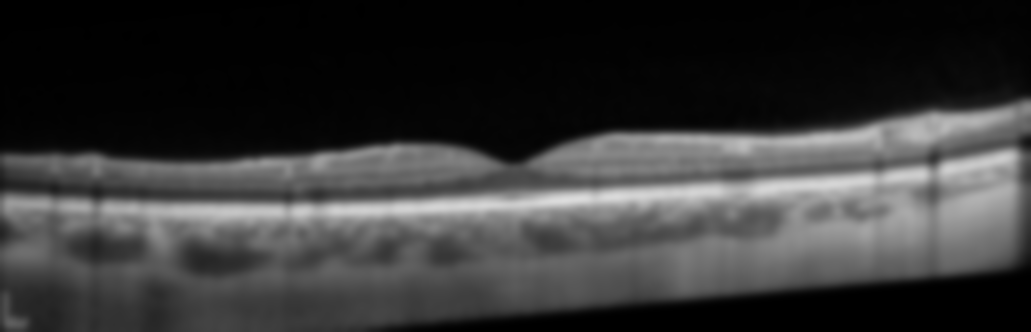
\includegraphics[width=\textwidth]{imagenes/tecnicas/EjemploTecnicasBlurGaussian23x23.png}}
  \caption{Gaussian Blur}
\end{figure}


\subsection{Basado en la mediana}\label{tecnica:blur-median}
En el caso de un \emph{median Blur} y como oposición al \emph{Blur},
que se basa en la media, el \emph{median Blur} calcula el valor
del píxel central mediante la mediana de los píxeles colindantes. \\
Esta técnica es muy útil para reducir el ruido granulado de la imagen.\\
En el siguiente ejemplo se muestra un ejemplo aplicando un
\emph{kernel} de tamaño $23 \times 23$ mediante
\mintinline{python}{cv2.medianBlur()}\footnote{\url{http://docs.opencv.org/modules/imgproc/doc/filtering.html\#cv2.medianBlur}}:

\begin{figure}[H]
  \caption{Original}
  \centering \setlength\fboxsep{0pt} \setlength\fboxrule{0.5pt}
  \fbox{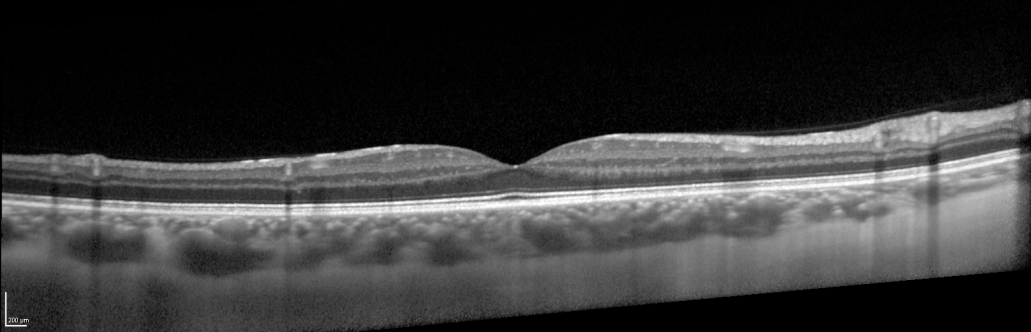
\includegraphics[width=\textwidth]{imagenes/tecnicas/EjemploTecnicasThresholdOriginal.png}}
\end{figure}

\begin{figure}[H]
  \centering \setlength\fboxsep{0pt} \setlength\fboxrule{0.5pt}
  \fbox{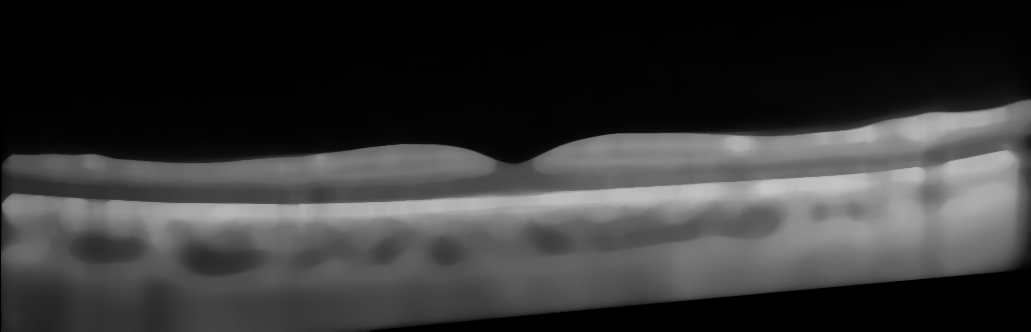
\includegraphics[width=\textwidth]{imagenes/tecnicas/EjemploTecnicasBlurMedian23.png}}
  \caption{Median Blur}
\end{figure}

\section{Transformaciones morfológicas}
Las operaciones de transformación morfológicas~\emph{\citep*[9
  Morphology]{fisher1996hypermedia}}~\emph{\citep*[Image
  Morphology]{opencv_book-bib}} se aplican sobre la forma de la
imagen. Se suelen usar para reducir el ruido, aislar o juntar
elementos. El \emph{kernel} aplicado a la imagen define el
resultado de la operación. \\
Normalmente, este tipo de operaciones se realizan posteriormente a una
operación de \emph{threshold} por lo que para entender mejor la
operación supondremos que la imagen está \emph{binarizada} (píxeles
únicamente blancos o negros). \\
A diferencia de los \emph{kernel} de convolución, los \emph{kernel}
morfológicos no necesitan ser de dimensión cuadrada ni contener
valores numéricos porque se utilizan como referencia para indicar las
posiciones de los píxeles.

\subsection{\emph{Erosion}}
Es una técnica que usa un \emph{kernel} a modo de máscara, sustituye
el píxel central por el \emph{mínimo local} de sus vecinos. Si algún
vecino es un píxel negro, automáticamente el píxel central se
convertirá en negro. El nombre procede del efecto que produce en una
imagen un artefacto blanco sobre fondo negro dando la sensación de
reducción del artefacto y reduciendo sus salientes. La fórmula es:
\begin{equation*}
  erode(x, y) = \min_{\substack{(x', y' \in \; kernel)}} imagen(x + x', y + y')
\end{equation*}
El siguiente ejemplo muestra el efecto de someter una imagen a una
operación de \emph{Erosion} con un \emph{kernel} de $5 \times 5$ todo
de unos mediante \mintinline{python}{cv2.erode()}\footnote{\url{http://docs.opencv.org/modules/imgproc/doc/filtering.html\#cv2.erode}}.

\begin{figure}[H]
  \caption{Original}
  \centering \setlength\fboxsep{0pt} \setlength\fboxrule{0.5pt}
  \fbox{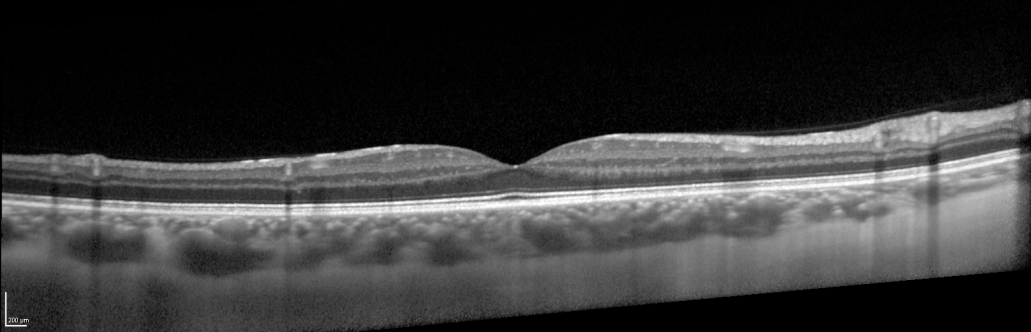
\includegraphics[width=\textwidth]{imagenes/tecnicas/EjemploTecnicasThresholdOriginal.png}}
\end{figure}

\begin{figure}[H]
  \centering \setlength\fboxsep{0pt} \setlength\fboxrule{0.5pt}
  \fbox{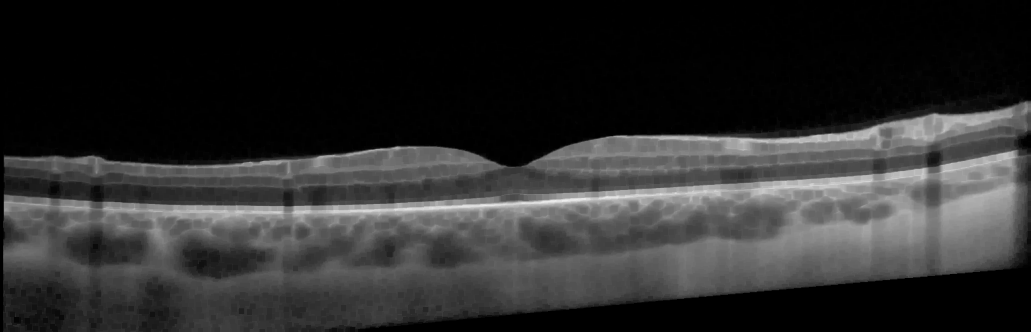
\includegraphics[width=\textwidth]{imagenes/tecnicas/EjemploTecnicasErosion.png}}
  \caption{Erosion}
\end{figure}


\subsection{\emph{Dilation}}\label{tecnica:dilation}
Es la técnica inversa a \emph{Erosion}, de la misma manera un
\emph{kernel} a modo de máscara sustituye el píxel central por el
\emph{máximo local}. Si alguno de sus vecinos es un píxel blanco, el
central automáticamente se convertirá en blanco. Igualmente, el nombre
procede del efecto que produce en una imagen con un artefacto blanco
sobre fondo negro dando la sensación de la dilatación del artefacto y
reduciendo sus concavidades. La fórmula es:
\begin{equation*}
  dilate(x, y) = \max_{\substack{(x', y' \in \;kernel)}} imagen(x + x', y + y')
\end{equation*}
El siguiente ejemplo muestra el efecto de someter una imagen a una
operación de \emph{Dilation} con un \emph{kernel} de $5 \times 5$ todo
de unos mediante
\mintinline{python}{cv2.dilate()}\footnote{http://docs.opencv.org/modules/imgproc/doc/filtering.html\#cv2.dilate}.

\begin{figure}[H]
  \caption{Original}
  \centering \setlength\fboxsep{0pt} \setlength\fboxrule{0.5pt}
  \fbox{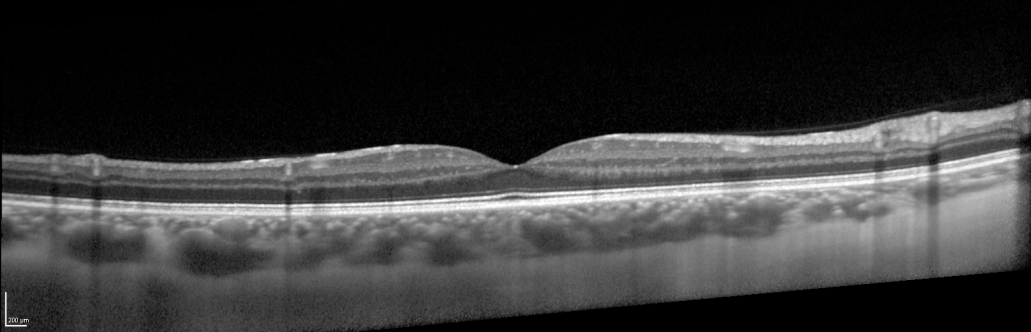
\includegraphics[width=\textwidth]{imagenes/tecnicas/EjemploTecnicasThresholdOriginal.png}}
\end{figure}

\begin{figure}[H]
  \centering \setlength\fboxsep{0pt} \setlength\fboxrule{0.5pt}
  \fbox{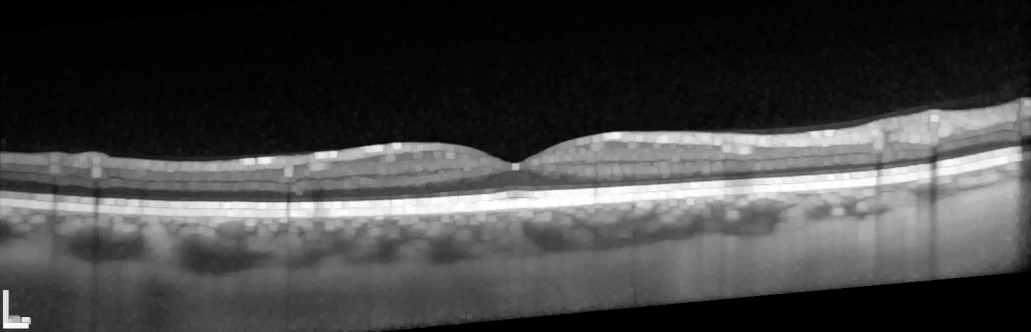
\includegraphics[width=\textwidth]{imagenes/tecnicas/EjemploTecnicasDilation.png}}
  \caption{Dilation}
\end{figure}

\subsection{\emph{Opening}}
La técnica de \emph{Opening} consiste en la realización de un
\emph{Erode} seguido de un \emph{Dilate}. Se utiliza para la
eliminación de ruido granulado alrededor del artefacto.\\
En el siguiente ejemplo se somete a la imagen a un \emph{Opening} con
\emph{kernel} de tamaño $9 \times 9$ mediante
\mintinline{python}{cv2.morphologyEx()}\footnote{\url{http://docs.opencv.org/modules/imgproc/doc/filtering.html\#cv2.morphologyEx}}.

\begin{figure}[H]
  \caption{Original}
  \centering \setlength\fboxsep{0pt} \setlength\fboxrule{0.5pt}
  \fbox{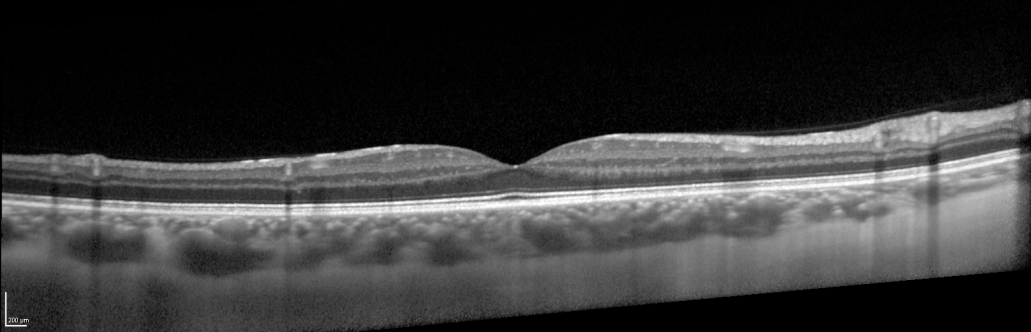
\includegraphics[width=\textwidth]{imagenes/tecnicas/EjemploTecnicasThresholdOriginal.png}}
\end{figure}

\begin{figure}[H]
  \centering \setlength\fboxsep{0pt} \setlength\fboxrule{0.5pt}
  \fbox{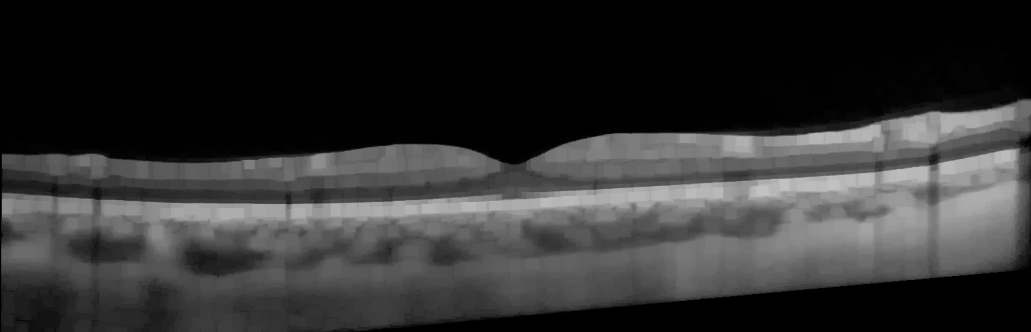
\includegraphics[width=\textwidth]{imagenes/tecnicas/EjemploTecnicasOpening9.png}}
  \caption{Opening}
\end{figure}

\subsection{\emph{Closing}}
La técnica de \emph{Closing} consiste en la realización de un
\emph{Dilate} seguido de un \emph{Erode}. Se utiliza para la
eliminación de ruido granulado situado en el interior del
artefacto. \\
En el siguiente ejemplo se somete a la imagen a un \emph{Closing} con
\emph{kernel} de tamaño $9 \times 9$ mediante
\mintinline{python}{cv2.morphologyEx()}\footnote{\url{http://docs.opencv.org/modules/imgproc/doc/filtering.html\#cv2.morphologyEx}}.

\begin{figure}[H]
  \caption{Original}
  \centering \setlength\fboxsep{0pt} \setlength\fboxrule{0.5pt}
  \fbox{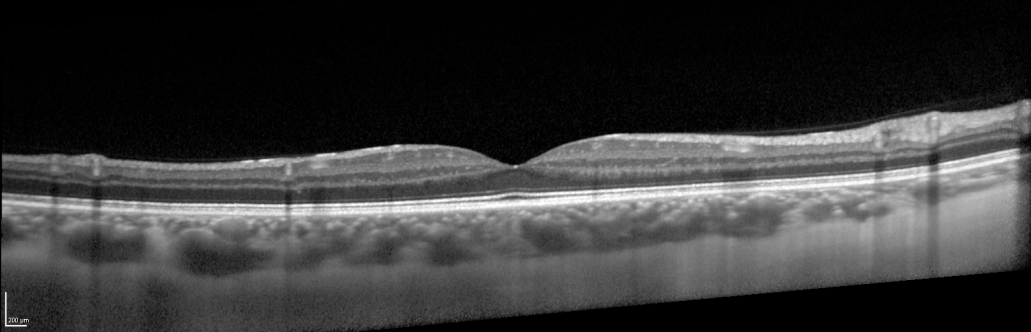
\includegraphics[width=\textwidth]{imagenes/tecnicas/EjemploTecnicasThresholdOriginal.png}}
\end{figure}

\begin{figure}[H]
  \centering \setlength\fboxsep{0pt} \setlength\fboxrule{0.5pt}
  \fbox{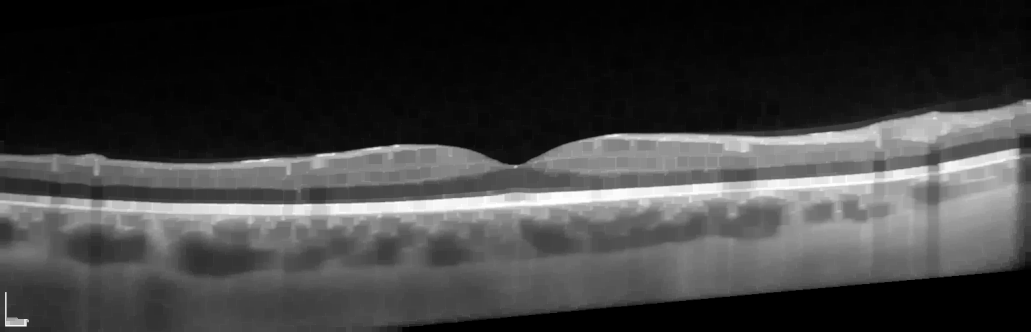
\includegraphics[width=\textwidth]{imagenes/tecnicas/EjemploTecnicasClosing9.png}}
  \caption{Opening}
\end{figure}

\subsection{Gradiente morfológico}
Es la diferencia entre la operación \emph{Dilation} y la operación
\emph{Erode} de la imagen. Se utiliza para marcar el perímetro o borde
del artefacto. La expresión es:
\begin{equation*}
  gradiente(imagen) = dilate(imagen) - erode(imagen)
\end{equation*}

\begin{figure}[H]
  \caption{Original}
  \centering \setlength\fboxsep{0pt} \setlength\fboxrule{0.5pt}
  \fbox{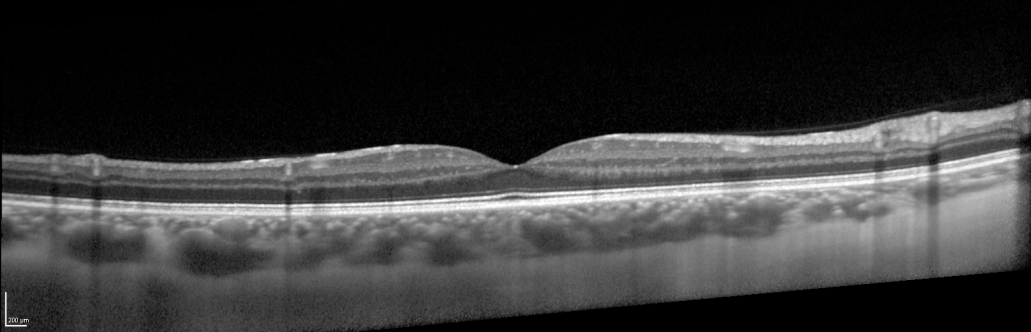
\includegraphics[width=\textwidth]{imagenes/tecnicas/EjemploTecnicasThresholdOriginal.png}}
\end{figure}

\begin{figure}[H]
  \centering \setlength\fboxsep{0pt} \setlength\fboxrule{0.5pt}
  \fbox{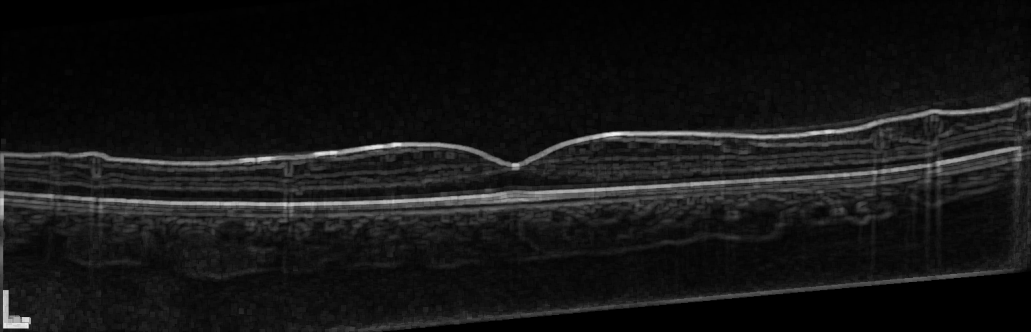
\includegraphics[width=\textwidth]{imagenes/tecnicas/EjemploTecnicasGradient.png}}
  \caption{Gradiente morfológico}
\end{figure}

\section{Gradientes}
El cálculo de gradientes o bordes \emph{\citep*[11. Feature
  Detectors]{fisher1996hypermedia}} \emph{\citep*[Gradients and Sobel
  Derivatives]{opencv_book-bib}} \emph{\citep*[5.1 Edge
  Tracking]{toennies2012guide}} se realiza mediante la convolución de
derivadas parciales del estilo:
\begin{equation*}
  \frac{\delta^{2}}{\delta x \delta y}
\end{equation*}
Por simplificación y eficiencia nos centraremos en describir sus
aproximaciones, más fáciles de entender. \\
El origen de los números de los \emph{kernels} se basa en el siguiente
proceso:\\
Una imagen se puede representar como una función de una señal continua
y discreta. Nos centraremos en ver el proceso con una fila de píxeles
de la imagen. Un borde es un cambio de color que en la función está
representado como un cambio de valor entre una posición y
otra. Matemáticamente, la manera de medir cuánto cambia entre un punto
,por ejemplo $x$, y otro muy próximo, $x + \delta x$, se realiza
mediante la
derivación.\\
La fórmula para derivar una imagen $I$ que sólo contenga una fila de
píxeles es la siguiente:
\begin{equation*}
  I'_x(x) = \lim_{\delta x \to 0}\frac{I(x+\delta x) - I(x)}{\delta x}
\end{equation*}
Como sólo se pueden computar valores discretos, el punto de la función
más cercano a $0$ es $\delta x = 1$. Esto aproxima la derivada a
\begin{equation*}
  I_x'(x) \approx I(x + 1) - I(x)
\end{equation*}
Si extraemos los coeficientes de las imágenes a un \emph{kernel}, el
resultado es:
\begin{equation*}
  kernel = \begin{bmatrix}
    1 & -1
  \end{bmatrix}
\end{equation*}
Nótese que la suma de todos los coeficientes siempre será $0$. Para
alargar el \emph{kernel} y abarcar más píxeles, por ejemplo tres, se
procede a introducir $0$ entre medias dando lugar a
$\begin{bmatrix} 1 & 0 & -1 \end{bmatrix}$ \\
Al realizar la primera derivada, nos encontramos que para interpretar
el gradiente tiene que ser un máximo local y suficientemente alto para
distinguirlo. Por lo que si aplicamos la segunda derivada suavizamos
el gradiente y obtenemos, de manera precisa, el máximo local, porque
toma el valor $0$ en el eje de abcisas. Si alargamos el \emph{kernel}
en los ejes $x, y$ obtendremos el \emph{kernel}
\emph{Sobel} que se explicará con detenimiento en el siguiente apartado. \\
La segunda derivada viene dada por:
\begin{equation*}
  I''(x) = \lim_{\delta x \to 0}\frac{I'(x+\delta x) - I'(x)}{\delta x}
\end{equation*}
Si aproximamos como la vez anterior $\delta x = 1$ obtenemos
\begin{equation*}
  I_x''(x) \approx I'(x + 1) - I'(x)
\end{equation*}
Como ya hemos aproximado la primera derivada:
\begin{equation*}
  I'(x) \approx I(x + 1) - I(x)
\end{equation*}
Podemos aplicarla a la segunda
\begin{equation*}
  I''(x) \approx \underbrace{I'(x + 1)}_{I(x + 2) - I(x + 1)} - \underbrace{I'(x)}_{I(x + 1) - I(x)}
\end{equation*}
Dando como resultado:
\begin{equation*}
  I''(x) \approx I(x) - 2I(x + 1) + I(x + 2)
\end{equation*}
Y al \emph{kernel} $\begin{bmatrix} 1 & -2 & 1 \end{bmatrix}$ que si
se expande en dos direcciones del espacio se obtiene el \emph{kernel
  Sobel} explicado en el apartado siguiente.\\
Imagen extraída de \emph{\citep*{opencv_book-bib}}~\footnote{Derecho
  de
  cita e ilustración de la enseñanza\\
  \url{http://www.riate.org/version/v1/recursos/cursolicenciasnavegable/derecho_de_cita_e_ilustracin_de_la_enseanza.html}\\
  \url{http://www.boe.es/boe/dias/2006/07/08/pdfs/A25561-25572.pdf}} a
modo de ejemplo para ilustrar primera y segunda derivada de un
gradiente.

\begin{figure}[H]
  \caption{Derivadas de un gradiente}
  \centering \setlength\fboxsep{0pt} \setlength\fboxrule{0.5pt}
  \fbox{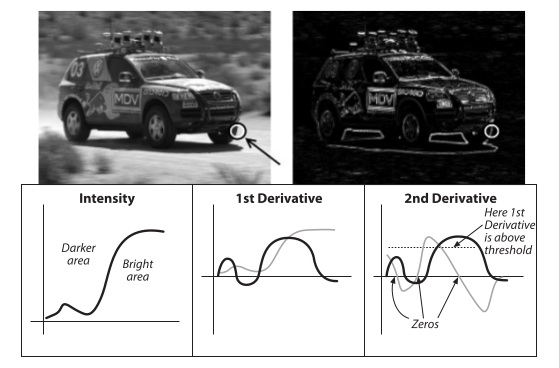
\includegraphics[width=\textwidth]{imagenes/tecnicas/derivatives.png}}
\end{figure}

\subsection{Sobel}
Como el operador \emph{Sobel} \emph{\citep*[History and definition of
  the sobel operator]{sobel2014history}} está definido en un espacio
discreto no es exactamente una derivada, representa un polinomio y la
segunda derivada, una función parabólica. Por esta razón, cuanto más
grande y más píxeles abarque el \emph{kernel} mejor aproximación se
obtiene y más tolerancia al ruido. Se aplica con
\mintinline{python}{cv2.Sobel()}\footnote{\url{http://docs.opencv.org/modules/imgproc/doc/filtering.html\#cv2.Sobel}}.
\begin{center}
  $ G_x = \begin{bmatrix}
    -1 & 0 & +1 \\
    -2 & 0 & +2 \\
    -1 & 0 & +1 \\
  \end{bmatrix}
  \hspace{0.5cm} \text{ y } \hspace{0.5cm} G_y = \begin{bmatrix}
    -1 & -2 & -1 \\
    0 & 0 & 0 \\
    +1 & +2 & +1 \\
  \end{bmatrix}
  $
  \\[0.5cm]
  $G = \sqrt{G_x\,^2 + G_y\,{2}}$
  \\[0.5cm]
  $\Theta= \arctan\left(\frac{G_y}{G_x} \right)$
\end{center}
La aproximación con el \emph{kernel} se hace de la siguiente manera:
\begin{equation*}
  Sobel(imagen) = \frac{\delta^{orden_x + orden_y} imagen}{\delta x^{orden_x} \delta
    y^{orden_y}} \text{ siendo el orden de derivación } orden_y \text{ y } orden_y > 0
\end{equation*}

\begin{figure}[H]
  \caption{Original}
  \centering \setlength\fboxsep{0pt} \setlength\fboxrule{0.5pt}
  \fbox{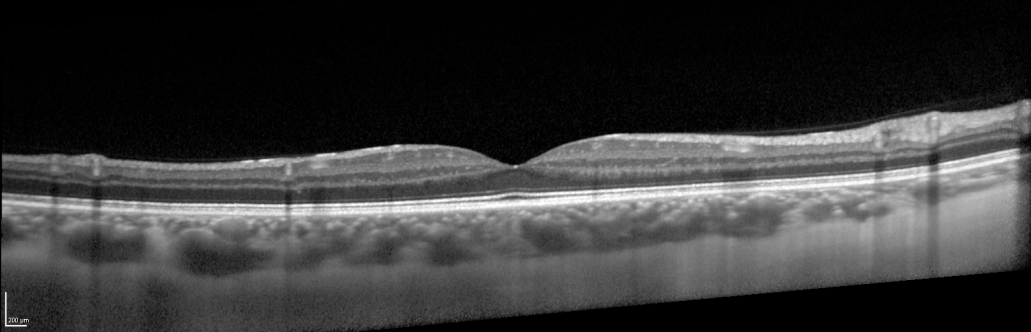
\includegraphics[width=\textwidth]{imagenes/tecnicas/EjemploTecnicasThresholdOriginal.png}}
\end{figure}

\begin{figure}[H]
  \centering \setlength\fboxsep{0pt} \setlength\fboxrule{0.5pt}
  \fbox{\includegraphics[width=\textwidth]{imagenes/tecnicas/EjemploTecnicasSobel.png}}
  \caption{Sobel}
\end{figure}

\subsection{Scharr}
El operador \emph{Scharr} se utiliza como el sustituto del operador
\emph{Sobel} cuando es necesario aplicar \emph{kernels} pequeños,
especialmente de tamaño $3 \times 3$, en los cuales al tener tan pocos
píxeles, los bordes no suelen estar posicionados sobre los ejes $x$ e
$y$ como en la superficie de los \emph{kernel} de gran tamaño por lo
que la aproximación de \emph{Sobel} es bastante inexacta con los
gradientes en forma de ángulo. Se aplica con
\mintinline{python}{cv2.Scharr}\footnote{\url{http://docs.opencv.org/modules/imgproc/doc/filtering.html\#cv2.Scharr}}.
\begin{center}
  $ G_x = \begin{bmatrix}
    +3 & 0 & -3 \\
    +10 & 0 & -10 \\
    +3 & 0 & -3 \\
  \end{bmatrix}
  \hspace{0.5cm} \text{ y } \hspace{0.5cm} G_y = \begin{bmatrix}
    +3 & +10 & +10 \\
    0 & 0 & 0 \\
    -3 & -10 & -10 \\
  \end{bmatrix}
  $
\end{center}

\begin{figure}[H]
  \caption{Original}
  \centering \setlength\fboxsep{0pt} \setlength\fboxrule{0.5pt}
  \fbox{\includegraphics[width=\textwidth]{imagenes/tecnicas/EjemploTecnicasThresholdOriginal.png}}
\end{figure}

\begin{figure}[H]
  \centering \setlength\fboxsep{0pt} \setlength\fboxrule{0.5pt}
  \fbox{\includegraphics[width=\textwidth]{imagenes/tecnicas/EjemploTecnicasScharr.png}}
  \caption{Scharr}
\end{figure}

\subsection{Laplaciano}
El operador \emph{Laplaciano} se define como la segunda derivada del
operador \emph{Sobel} de la siguiente manera usando
\mintinline{python}{cv2.Laplacian()}\footnote{\url{http://docs.opencv.org/modules/imgproc/doc/filtering.html\#cv2.Laplacian}}
\begin{equation*}
  Laplaciana(imagen) = \frac{\delta^{2} imagen}{\delta x^{2}} + \frac{\delta^{2} imagen}{\delta y^{2}}
\end{equation*}
Por motivos de eficiencia, se aproxima con el \emph{kernel} siguiente
\begin{center}
  $ kernel = \begin{bmatrix}
    0 & +1 & 0 \\
    +1 & -4 & +1 \\
    0 & +1 & 0 \\
  \end{bmatrix}
  $
\end{center}

\begin{figure}[H]
  \caption{Original}
  \centering \setlength\fboxsep{0pt} \setlength\fboxrule{0.5pt}
  \fbox{\includegraphics[width=\textwidth]{imagenes/tecnicas/EjemploTecnicasThresholdOriginal.png}}
\end{figure}

\begin{figure}[H]
  \centering \setlength\fboxsep{0pt} \setlength\fboxrule{0.5pt}
  \fbox{\includegraphics[width=\textwidth]{imagenes/tecnicas/EjemploTecnicasLaplacian.png}}
  \caption{Laplaciano}
\end{figure}

\section{Algoritmo \emph{Canny}}\label{tecnica:canny}
El \emph{Canny} \emph{\citep*[A computational approach to edge
  detection]{canny1986computational}}
\emph{\citep*[Canny]{opencv_book-bib}} \emph{\citep*[5.1 Edge
  Tracking]{toennies2012guide}} es un algoritmo de detección de bordes
conocido como el \emph{detector óptimo} con la función de satisfacer
tres criterios principales:
\begin{itemize}
\item Bajo índice de error.
\item Minimización de la distancia entre los bordes detectados y los
  reales.
\item Un único detector por borde.
\end{itemize}
Para ello lo primero que hace es descartar el ruido usando el filtro
Gaussiano.
El \emph{kernel} usado para este filtro no es fijo.\\
Luego encuentra la intensidad del gradiente de la imagen con
procedimiento similar al Sobel con las mismas máscaras de convolución,
fuerza del gradiente y dirección.\\
Posteriormente, se suprimen los píxeles que no se consideran parte del
borde de forma que solo queden unas finas líneas. Estas líneas son los posibles bordes.\\
Por último, se usan dos \emph{thresholds}, uno alto y uno bajo: Si el
gradiente del píxel es mayor que el threshold alto, el píxel formará
parte del borde; si el gradiente del píxel es menor que el threshold
bajo, no se tendrá en cuenta; en caso de que el gradiente del píxel
esté entre ambos \emph{thresholds} se considerará solo si está
contiguo a un píxel cuyo gradiente sea superior al threshold alto.\\
El siguiente ejemplo muestra el resultado de aplicar \emph{Canny} a
una imagen mediante
\mintinline{python}{cv2.Canny()}\footnote{\url{http://docs.opencv.org/modules/imgproc/doc/feature\_detection.html\#cv2.Canny}}.

\begin{figure}[H]
  \caption{Original}
  \centering \setlength\fboxsep{0pt} \setlength\fboxrule{0.5pt}
  \fbox{\includegraphics[width=\textwidth]{imagenes/tecnicas/EjemploTecnicasThresholdOriginal.png}}
\end{figure}

\begin{figure}[H]
  \centering \setlength\fboxsep{0pt} \setlength\fboxrule{0.5pt}
  \fbox{\includegraphics[width=\textwidth]{imagenes/tecnicas/EjemploTecnicasCanny.png}}
  \caption{Canny}
\end{figure}

\section{Transformada de \emph{Hough}}\label{tecnica:hough}
La transformada de \emph{Hough} \emph{\citep*[Use of the hough
  trasformtion to detect lines and curves in pictures]{hart1971use}}
\emph{\citep*[4.3.2 Hough transforms]{szeliski2010computer}}
\emph{\citep*[5.2 Hough Transform]{toennies2012guide}} es una técnica
que se aplica para encontrar formas en una imagen \emph{binarizada} o
tras haber aplicado un algoritmo de detección de bordes y contornos
como el \emph{Canny}, incluso aunque haya ruido, siempre que se puedan
expresar matemáticamente como líneas rectas y curvas. Nos centraremos
sólo en explicar con rectas.
\subsection{Rectas}
Cualquier punto obtenido de una imagen puede formar parte de una línea
recta. Representamos una recta de manera simplificada como
\begin{equation*}
  y = mx + c
\end{equation*}
O mejor, de forma paramétrica porque al pasar infinitas rectas por un
punto lo más sencillo es limitar a un rango de ángulos.
\begin{equation*}
  \rho = x \cos \theta + y \sin \theta
\end{equation*}
donde $\rho$ es la distancia perpendicular a la recta desde el origen y
$\theta$ el ángulo que forman la recta de la distancia con el
origen. En \emph{OpenCV} el origen está situado en la parte superior
izquierda. Si la recta a dibujar corta al eje de abcisas con un valor
positivo el ángulo $\theta$ es menor que $180º$ y el valor de $\rho$
es positivo. Por el contrario, si corta al eje de abcisas por un valor
negativo, el ángulo $\theta$ es mayor de $180º$ y $\rho$ es
negativo. Los casos extremos son las líneas verticales $0º$ y
horizontales $90º$.\\
Por claridad, imaginemos sólo dos puntos [\emph{figura~\ref{fig:hough}
  a)}] por los que queremos trazar una recta. Para ello, trazaremos
tantas rectas como $\theta$ determinemos por cada punto
[\emph{figura~\ref{fig:hough} b)}], almacenando de cada uno su
$\theta$ y su $\rho$. Con estos pares, se construye una gráfica donde
el eje $y$ de ordenadas sea $\rho$ y el eje $x$ de abcisas sea
$\theta$. Cada punto genera una curva [\emph{figura~\ref{fig:hough}
  c)}] y en el punto de intersección de las dos encontramos la
$\theta$ y $\rho$ de la recta que pasa por los dos puntos. Por
supuesto, \emph{OpenCV} no calcula la gráfica sino que guarda los
pares y acumula el número de apariciones de cada uno y finalmente
devuelve el máximo local.

\begin{figure}[H]
  \caption{Transformada de Hough}
  \centering \setlength\fboxsep{0pt} \setlength\fboxrule{0.5pt}
  \fbox{\includegraphics[width=\textwidth]{imagenes/tecnicas/houghTransform.png}}\label{fig:hough}
\end{figure}

Imagen extraída de \emph{\citep*{opencv_book-bib}}~\footnote{Derecho
  de
  cita e ilustración de la enseñanza\\
  \url{http://www.riate.org/version/v1/recursos/cursolicenciasnavegable/derecho_de_cita_e_ilustracin_de_la_enseanza.html}\\
  \url{http://www.boe.es/boe/dias/2006/07/08/pdfs/A25561-25572.pdf}}

Ejemplo de una recta de \emph{Hough} obtenida con
\mintinline{python}{cv2.HoughLines()}\footnote{\url{http://docs.opencv.org/modules/imgproc/doc/feature\_detection.html\#cv2.HoughLines}}
tras la aplicación de un \emph{Canny}.

\begin{figure}[H]
  \caption{Original}
  \centering \setlength\fboxsep{0pt} \setlength\fboxrule{0.5pt}
  \fbox{\includegraphics[width=\textwidth]{imagenes/tecnicas/EjemploTecnicasThresholdOriginal.png}}
\end{figure}

\begin{figure}[H]
  \centering \setlength\fboxsep{0pt} \setlength\fboxrule{0.5pt}
  \fbox{\includegraphics[width=\textwidth]{imagenes/tecnicas/EjemploTecnicasHough.png}}
  \caption{Recta de Hough}
\end{figure}

\section{Contornos}\label{tecnica:contornos}
Un contorno es una línea curva formada por la únión de puntos que
tienen el mismo color o intensidad. La detección de contornos
\emph{\citep*[Contours in OpenCV]{opencv_tutorial-bib}}
\emph{\citep*[5.1 Edge Tracking]{toennies2012guide}}se usa para
estudiar la forma de los artefactos de la imagen. \emph{OpenCV}
entiende detectar contornos como la búsqueda de artefactos blancos
sobre un fondo negro por lo que la imagen, tiene que ser previamente
\emph{binarizada}. Normalmente, se preprocesa con la aplicación de un
\emph{Canny} o similar y una vez obtenidos los contornos se almacenan
en una estructura de árbol para indicar los contornos que están dentro
de otros. \\
Por esta razón, siempre que se pueda, es recomendable usar un
algoritmo de detección de contornos para luego filtrarlos y/o
tratarlos individualmente en vez de un algoritmo de detección de
gradientes o de tipo \emph{Canny}.\\
Estos algoritmos están divididos en dos partes:
\begin{description}
\item[Detección:] parte encargada de la búsqueda y jerarquización de
  los contornos.
\item[Dibujado:] parte encargada del coloreado y grosor de las líneas.
\end{description}

Ejemplo obtenido tras aplicar esta técnica con
\mintinline{python}{cv2.findContours()}\footnote{\url{http://docs.opencv.org/modules/imgproc/doc/structural\_analysis\_and\_shape\_descriptors.html\#cv2.findContours}}
y
\mintinline{python}{cv2.drawContours()}\footnote{\url{http://docs.opencv.org/modules/imgproc/doc/structural\_analysis\_and\_shape\_descriptors.html\#cv2.drawContours}}
para su visualización.

\begin{figure}[H]
  \caption{Original}
  \centering \setlength\fboxsep{0pt} \setlength\fboxrule{0.5pt}
  \fbox{\includegraphics[width=\textwidth]{imagenes/tecnicas/EjemploTecnicasThresholdOriginal.png}}
\end{figure}

\begin{figure}[H]
  \centering \setlength\fboxsep{0pt} \setlength\fboxrule{0.5pt}
  \fbox{\includegraphics[width=\textwidth]{imagenes/tecnicas/EjemploTecnicasFindcontours.png}}
  \caption{Contornos}
\end{figure}

\section{Puntos de interés o \emph{Blobs}}\label{tecnica:blobs}
Las bibliotecas de visión computarizada proporcionan numerosas
técnicas de detección de gradientes, contornos y algoritmos de tipo
\emph{Canny}. Además, traen abstracciones de alto nivel para la
detección de \emph{Blobs} o puntos de interés \emph{\citep*[1.7 Blob
  Detection]{simplecv_book-bib}} \emph{\citep*[5.4
  Blobs]{toennies2012guide}}.\\
La detección de \emph{Blobs} es el siguiente paso de abstracción
después de la detección de contornos. Un \emph{Blob} es una región
blanca en una imagen previamente \emph{binarizada}. \\
\emph{OpenCV} carece de esta abstracción, siendo necesario usar la
biblioteca \emph{SimpleCV}. Explicar su funcionamiento requiere la
descripción de su código en los siguientes pasos:
\begin{enumerate}
\item Se realiza una \emph{binarización} a la imagen mediante un
  \emph{threshold}, que puede ser con un valor umbral fijo o, por el
  contrario, un \emph{threshold adaptativo}. La implementación en este
  caso aplica \emph{Otsu}.
\item Se utiliza el algoritmo de detección de contornos anteriormente
  explicado.
\item Se analizan los contornos encontrados:
  \begin{enumerate}[label*=\arabic*.]
  \item\label{paso:contornos} Si es un hueco, se descarta y se pasa al
    siguiente contorno. En caso contrario, se devuelven sus
    propiedades. Las propiedades más importantes son:
    \begin{description}
    \item[Área]
    \item[Perímetro]
    \item[Contorno]
    \item[Contorno convexo]
    \item[Rectángulo rellenado]
    \item[Los 7 momentos de \emph{Hu}:] los momentos
      \emph{\citep*[Visual pattern recognition by moment
        invariants]{hu1962visual}} son varios cálculos distintos de
      alta complejidad para determinar de manera inequívoca al
      \emph{Blob} como si de un invariante se tratase ante cambios de
      escala, rotación o ambos.\footnote{Los momentos de una imagen se
        han dejado sin explicar en profundidad porque su descripción
        no es relevante para el entendimiento del algoritmo.}
    \end{description}
  \item Si hay un contorno interno, se almacena para procesarlo
    posteriormente.
  \item Se procede a analizar el siguiente contorno externo volviendo
    al paso~\ref{paso:contornos} hasta que no quede ninguno.
  \end{enumerate}
\item Se procede a analizar todos los contornos internos almacenados
  uno a uno volviendo al paso~\ref{paso:contornos} de manera
  recursiva.
\item Finalmente, el algoritmo devuelve una lista con todos los
  \emph{Blobs} detectados ordenados de menor a mayor área (por la
  manera recursiva en la que se procesaron de más externos a más
  internos).
\end{enumerate}

Ejemplo detección de \emph{blobs} con área máxima de $20.000$ píxeles
y negros por lo que, previamente, se realizó una \emph{binarización
  inversa} y finalmente
\mintinline{python}{findBlobs()}\footnote{\url{https://github.com/sightmachine/SimpleCV/blob/6c4d61b6d1d9d856b471910107cad0838954d2b2/SimpleCV/ImageClass.py\#L3422}}
para detectarlos.

\begin{figure}[H]
  \caption{Original}
  \centering \setlength\fboxsep{0pt} \setlength\fboxrule{0.5pt}
  \fbox{\includegraphics[width=\textwidth]{imagenes/tecnicas/EjemploTecnicasThresholdOriginal.png}}
\end{figure}

\begin{figure}[H]
  \centering \setlength\fboxsep{0pt} \setlength\fboxrule{0.5pt}
  \fbox{\includegraphics[width=\textwidth]{imagenes/tecnicas/EjemploTecnicasBlobs.png}}
  \caption{Blobs}
\end{figure}

\part{Investigación}
\chapter{Tomografías de Coherencia Óptica}
Toda la información de este capítulo ha sido cuidadosamente
seleccionada y adaptada de \emph{Avances en la exploración de la
  retina: OCT:\@ Qué es y para qué sirve}~\citep*{oct-bib}

\section{Imágenes TCO}
Las \gls{tco} son un tipo de imágenes ampliamente utilizadas en el
ámbito hospitalario por los oftalmólogos para estudiar, explorar y
monitorizar las estructuras oculares de los pacientes para el
diagnóstico de enfermedades, especialmente, de difícil identificación
oftalmológica.

\section{Máquina de TCO}
Una máquina de \gls{tco} se utiliza para la exploración en tiempo real,
sin ser invasiva ni dolorosa, para obtener con resolución micrométrica
imágenes de estructuras de tejidos vivos. Con el paso del tiempo se ha
hecho insustituible en el diagnóstico y seguimiento de numerosas
patologías oculares, así como también por la mejora de su rapidez y
precisión.

\subsection{Propiedades ópticas de los tejidos}
La máquina de \gls{tco} es capaz de medir y representar los distintos
tipos de tejidos en escala de grises o colores según su reflectividad:
\begin{description}
\item[Reflectividad alta:] sangre, exudados lipídicos, epitelio
  pigmentario, coriocapilar o capas de fibras nerviosas
  perpendiculares al haz de luz. Representados con colores cálidos
  como rojo y blanco.
\item[Reflectividad media:] capas retinianas de la limitante interna a
  la plexiforme externa. Representadas con colores verdes y amarillos
\item[Reflectividad baja:] zonas de edema, vítreo y contenido seroso,
  dispuestos en paralelo al haz de luz. Representados con colores
  fríos como azul y negro.
\end{description}

\subsection{Base teórica}
La máquina de \gls{tco} usa una técnica análoga a las máquina de
ecografías pero sustituyendo los ultrasonidos por luz. La máquina mide
la latencia o retardo e intensidad de la onda reflejada tras incidir
en un tejido. La ventaja de una máquina de \gls{tco} frente a una de
ecografías es la velocidad de la luz, muy superior a la velocidad de
los ultrasonidos, del orden de \emph{$10^{-15}$ fentosegundos},
requiriendo un sistema de medición indirecto.\\
\emph{El interferómetro de Michelson} es la principal base del
funcionamiento de estas máquinas. Consiste en dirigir la radiación a
un divisor de haces que a su vez los divide en dos. Un haz se dirige
por un medio conocido y el otro por el medio a estudiar. Tras esto,
ambos haces se reflejan para hacerlos coincidir en un mismo punto,
usando el haz que atraviesa el medio conocido como patrón para
registrar la interferencia entre ambos y medir la intensidad y el
retardo del haz que recorrió el medio desconocido.

\subsection{Historia}
Estas primeras máquinas operaban sobre el \emph{dominio temporal}. Es
decir, el haz se reflejaba sobre un espejo que se movía para para
recorrer todo el espacio a estudiar. La velocidad de traslación del
espejo se convertía en el factor crítico y limitante de la velocidad
de
captura. En los mejores casos se alcanzaban los \emph{400 barridos por segundo}.\\
La velocidad de barrido es crítica principalmente por dos motivos:
\begin{description}
\item [Disminución del tiempo de estudio] de la estructura
  ocular. Esto reduce la irritación y la sequedad del ojo del paciente
  que, al tenerlo abierto durante todo el proceso, hacen que se
  reduzca la calidad del resultado obtenido.
\item [La resolución y calidad] son directamente proporcionales número
  de muestras realizadas. Es decir, cuantos más barridos, mejores
  resultados pero aumentar el número de barridos también aumenta el
  tiempo de exploración, por lo que es necesario buscar un equilibrio
  entre la resolución y la duración de la exploración.
\end{description}
Con el paso del tiempo y el perfeccionamiento de la técnica, se hizo
posible fijar el espejo y aumentar así los barridos por segundo
mediante el uso del \emph{dominio espectral o de Fourier}. Esta
técnica se sustenta en una serie de dispositivos que analizan el haz a
comparar con el de referencia. Con el espejo fijo en un punto y los
nuevos dispositivos, se consiguió hacer los barridos hasta 700 veces
más rápido, alcanzando los \emph{25.000 barridos por segundo}.\\
Actualmente, las máquinas trabajan con una variante del \emph{dominio
  espectral}: las llamadas de tipo \emph{swept-source}. Estas utilizan
el dominio de la frecuencia codificada en el tiempo (\emph{Time
  encoded frequency domain}). Para ello, un láser sintonizable emite
el haz con una longitud de onda fija que muestrea secuencialmente el
medio con una serie de longitudes de onda individuales que
posteriormente descodifica. Así, alcanza una velocidad de
\emph{100.000 muestreos por segundo}. Además, proporciona imágenes muy
precisas y es capaz de explorar a todos los niveles de profundidad,
por lo que es capaz de mostrar simultáneamente (en la misma
exploración) imágenes de gran calidad tanto de estructuras
superficiales como el vítreo, como de las más profundas, como la
\emph{\gls{coroides}} e incluso la \emph{\gls{esclera}}.

\subsection{Tipo, resolución y densidad de muestreo}
\subsubsection{Tipo}
Para la reconstrucción de la imagen de un tejido, la máquina de \gls{tco}
explora el medio con un haz de luz en un punto o
\emph{\textbf{A-scan}}. La repetición de puntos sobre una misma línea
genera un plano denominado \emph{\textbf{B-scan}}. La repetición de
estos planos construye un cubo.
\subsubsection{Resolución}
La resolución de muestreo se define como la distancia mínima entre dos
puntos próximos distintos. Permite distinguir ambos puntos como
diferentes.
\begin{itemize}
\item Resolución \textbf{axial}: limitada por la longitud de
  coherencia de la onda.
\item Resolución \textbf{transversal}: dependiente de la anchura del
  haz de luz incidente.
\end{itemize}
\subsubsection{Densidad}
La densidad de muestreo se define como la cantidad de
\emph{\textbf{A-scan}} por unidad de volumen de tejido. Es
directamente proporcional al tiempo de exploración.

\subsection{Número de muestreos en el mismo punto o \emph{frame
    averaging}}
Para incrementar la calidad de una imagen es recomendable aumentar el
número de muestreos puesto que las máquinas de \gls{tco} usan luz
parcialmente coherente y las reflexiones adyacentes producen
interferencias o ruido en el tejido. Este ruido es siempre distinto en
cada exploración por lo que, al repetir el proceso en cada punto del
tejido y hacer su promedio para reconstruir la imagen, el ruido
desaparece. Esto hace posible distinguir capas con bajo contraste o
muy finas.\\
Aunque el aumento de muestreos a priori puede parecer una buena
técnica para mejorar la calidad, requiere incrementar
considerablemente el tiempo de exploración produciendo en el ojo del
paciente sequedad e irritación. Esto no sólo disminuye la calidad sino
que incluso puede llegar a impedir finalizar correctamente la
exploración. Por lo que hay que buscar un equilibrio entre número de
muestreos y tiempo de exploración.\\
La estimación de calidad-ruido se basa en la recomendación de
\emph{\textbf{100 muestreos de tipo B-scan}}, explicados
anteriormente.

\subsection{Tipos de exploración}
Lo habitual es la \emph{exploración lineal} porque son las más rápidas
de realizar y tolerables hasta para los ojos con
fatiga, habitual en las personas a partir de cierta edad.\\
La reconstrucción en 3D de estructuras oculares mediante cubos
proporciona mucha más información y permite seleccionar
individualmente cada corte o punto que se quiera
visualizar. Consecuentemente, alarga el proceso siendo inviable de
realizar a pacientes poco colaboradores o con ojos con tendencia a
secarse.\\
Es importante saber que aunque las zonas a explorar están
estandarizadas, cada máquina de \gls{tco} tiene su propia estrategia.

\subsection{Software de análisis de la información}
Un aspecto crítico de las máquinas de \gls{tco} es el software que
incorporan mediante algoritmos de segmentación para medir las
dimensiones de las estructuras previamente exploradas. Teniendo en
cuenta que al tener cada máquina su propia estrategia de exploración,
un mismo tejido en máquinas de \gls{tco} distintas proporciona medidas
diferentes.

\subsection{Seguimiento}
Las máquinas de \gls{tco} más modernas son capaces de reconocer la zona
que está siendo explorada a partir de características distintivas como
los bordes de la papila o vasos sanguíneos. Permite asegurar así con
exploraciones sucesivas a lo largo del tiempo de una misma zona que
los cambios detectados en un punto son reales y no artefactos de
puntos próximos y distintos.\\
Este seguimiento permite, además, medir la distancia entre los dos
mismos puntos en exploraciones sucesivas,lo cual permite cuantificar
los cambios que puedan producirse.

\subsection{Otras características}
La mayoría de las máquinas de \gls{tco} tienen por objetivo el segmento
anterior o el posterior, pero no los dos simultáneamente, ya que
las longitudes de onda idóneas para cada uno son diferentes.\\
Sin embargo, si se aleja la máquina del ojo, las ondas dirigidas al
segmento posterior también pueden usarse para explorar el segmento
anterior.

\subsection{Informes}
Las máquina de \gls{tco} emiten informes de todas las exploraciones de
uno o ambos ojos con múltiples parámetros. \emph{Informes de análisis}
sobre una única exploración o sobre diversas marcando los cambios. Con
algunas enfermedades además de un informe de análisis, se puede
generar un \emph{informe de evolución} acerca de la posible variación
en el tiempo del grosor de algunas capas.\\
Todos los informes han de ser valorados después de la exploración y
antes de ser tenidos en cuenta, de forma que se verifique la
corrección de sus datos, y que la exploración se ha realizado
correctamente y es fiable.

\section{Aplicaciones clínicas}
\begin{itemize}
\item Medición de grosores.
\item Visualización de alteraciones estructurales.
\item Medición de ángulos.
\end{itemize}
\chapter{Medición del espesor de la coroides}
\section{Problema}
Los estudios demuestran que hay una relación entre la inflamación de
la \emph{coroides} y la aparición de la \emph{uveítis}. Es necesario,
por tanto, medir el espesor de la coroides para prevenir esta
enfermedad y para seguir su evolución en el tiempo.\\
La \emph{coroides} o \emph{úvea} es una membrana por la que pasan gran
cantidad de vasos sanguíneos, cuya función es mantener la temperatura
constante y nutrir ciertas estructuras del globo ocular. \\
Gracias a las \gls{tco} es posible medir el grosor de la
membrana. Sin embargo, el software de la máquina no realiza la
medición de forma automática, sino que es necesario trazar la línea a
mano. Esto ralentiza el proceso y, además, genera imprecisiones en las
mediciones debidos principalmente a fallos humanos: Si la imagen no
está en posición horizontal es difícil trazar una línea perpendicular,
puede fallar el pulso, etc. Esta línea se debe trazar por el punto
menos profundo de la retina, conocido como \emph{fóvea} y de forma
perpendicular a la \emph{membrana de Bruch}. Una vez trazada la línea,
hay que medirla.


\section{Objetivos}
Los objetivos puestos en común después de sucesivas reuniones fueron:
\begin{itemize}
\item Automatizar lo máximo posible o requerir intervención mínima del
  oftalmólogo en el proceso de marcado de los puntos del espesor a medir de la
  \emph{coroides}.
\item Una vez delimitado el espesor de la \emph{coroides},
  proporcionar su medida en micras lo más fielmente posible.
\end{itemize}
Cumplir estos objetivos propuestos proporcionaría al estudio de la
evolución y control de la \emph{uveítis} una automatización completa
del seguimiento, pudiendo realizar las medidas de todo el historial de
un paciente en pocos segundos. Lo más importante no es el tiempo
ahorrado sino la erradicación de errores de precisión manuales y
resultados distintos de una misma imagen.

\section{Estudio}
El estudio se ha realizado en distintas fases, todas ellas de manera
secuencial y acumulativa. Además de la documentación de cada fase, se
proporcionan las mismas imágenes de guía y apoyo usadas durante el
estudio.  Sin embargo, aunque las fases aquí expuestas se encuentren
en orden secuencial, el orden cronológico en el que se resolvieron
varía, debido a que con cada nueva imagen que se estudiaba surgían
nuevos problemas.
\begin{enumerate}
\item El primer paso consistió en \textbf{extraer} de la imagen
  original \textbf{el área de interés}. Las máquinas \gls{tco}
  siempre proporcionan, además
  de la zona de estudio, el corte usado sobre la estructura ocular. \\
  \textbf{Se desarrolló una biblioteca encargada de automatizar la
    extracción del área de estudio.}
\item El corte programado durante la exploración tiene un grado de
  inclinación sobre la estructura ocular. \textbf{En la mayoría de las
    exploraciones el corte no es horizontal} o ,si se realizan
  exploraciones desde todos los ángulos, sólo uno muestra la estructura
  de manera horizontal. \\
  \textbf{Se desarrolló un algoritmo para la corrección de la
    inclinación} y así rotar la imagen el grado de desviación del
  corte con respecto a la horizontal de la estructura ocular.
\item Corregida la inclinación de la estructura y para poder realizar
  la medición de la \emph{coroides}, \textbf{es necesario} previamente
  \textbf{establecer un punto de referencia, la \emph{fóvea}}. \\
  \textbf{Se desarrolló un algoritmo para la detección del mínimo
    local de la superficie de la retina, la \emph{fóvea}.}
\item Una vez fijada la \emph{fóvea} \textbf{se marcan los dos puntos
    de la \emph{coroides} necesarios para poder medir su espesor}. \\
  \textbf{Se desarrolló un algoritmo para la detección de los puntos
    de espesor de la \emph{coroides}}
\item Finalmente, \textbf{se realiza la medición del espesor de la
    \emph{coroides}}. Este es el proceso más delicado e impreciso de
  todo el estudio porque al aplicar tantas técnicas de procesamiento a
  la imagen de manera consecutiva, hay que dar una medida en micras
  con el mínimo error de precisión posible del espesor de la \emph{coroides}. \\
  \textbf{Se desarrolló un algoritmo para la medición en micras del
    espesor de la \emph{coroides}}
\end{enumerate}


\section{Algoritmo propuesto}
\begin{enumerate}
\item La primera fase consistió en delimitar y extraer el área a
  investigar. Esto es así, porque las máquinas \gls{tco} en una misma
  imagen presentan el corte analizado y su resultado.\\
  Para resolver este problema de forma automática se procedió a
  realizar una biblioteca que realiza el siguiente procedimiento a la
  imagen.
  \begin{enumerate}[label*=\arabic*.]
  \item Convierte la imagen de escala \emph{RGB} a \emph{escala de
      grises}
  \item Duplica la imagen, en una aplica un \emph{threshold Otsu} y en
    otra un \emph{threshold binario} para \emph{binarizar} la imagen.
  \item Se recorre la imagen del \emph{threshold Otsu} con una
    horizontal de derecha a izquierda, desde la esquina superior
    derecha con las coordenadas, 0 como $x$ y ancho de la imagen como
    $y$ encontrar el borde de separación entre las dos imágenes.
  \item Al conocer el  \textbf{punto del borde de separación en la parte
    superior}, queda buscarlo también en la parte inferior de abajo a arriba en la
    imagen del \emph{threshold binario} con las coordenadas, el borde
    de separación como $x$ y la altura de la imagen como $y$.
  \item Con estos puntos ya se puede obtener la zona de la imagen
    original a estudiar. Si se apura y se recorta el negro sobrante de
    la parte inferior evita errores en la detección del segundo punto
    de la \emph{coroides} en algunos casos.
    \begin{enumerate}[label*=\arabic*.]
    \item Para eliminar dicha zona y como la imagen no tiene por qué
      estar en posición horizontal, se procede a buscar dos puntos
      auxiliares: uno empieza con la $x$ igual a $2/4$ de la anchura
      de la imagen, y el otro con la $x$ igual a $3/4$ de la
      anchura. Ambos empiezan con $y$ igual al borde inferior
      provisional hacia arriba, ignorando toda el área negra.
    \item Una vez obtenidos los dos puntos, se procede a obtener el
      punto definitivo para generar el rectángulo que contiene la
      imagen de estudio.
    \item Para calcular dicho punto, el que está situado más cerca del
      borde inferior para no recortar parte de la propia imagen si no
      está horizontal, hay que calcular primero otros dos. Esos puntos
      son la intersección de una recta imaginaria con los puntos
      auxiliares del paso anterior. Se calculan añadiendo a la $y$ de
      cada punto auxiliar la diferencia con respecto a la $y$ del otro
      punto auxiliar.
    \item Obtenidos estos dos puntos, el que tenga mayor $y$, es
      \textbf{el más cercano al borde inferior} y por tanto el
      utilizado como base para obtener el segundo punto del
      rectángulo.
    \item Finalmente, \textbf{se obtiene el rectángulo que contiene a}
      la parte de \textbf{la imagen} que queremos estudiar \textbf{con
        el punto del borde de separación de la parte superior y el
        punto} formado por la $y$ del punto \textbf{más cercano al
        borde inferior} del paso anterior y la anchura de la imagen
      original como la $x$.
    \end{enumerate}
  \end{enumerate}

\end{enumerate}
\chapter{Medición del área de los poros de la lámina cribosa}
\section{Problema}
En el curso de la investigación que se está llevando a cabo
actualmente sobre el \emph{\gls{glaucoma}} y las causas que lo
provocan, se ha detectado una posible relación con la aparición y
tamaño de los poros de la \emph{\gls{lamina-cribosa}} en la
\emph{\gls{papila-optica}} o cabeza del nervio óptico. \\
La \emph{\gls{papila-optica}} o \emph{disco óptico} es el punto donde
el nervio óptico entra en el globo ocular. Tiene la forma de un
pequeño disco rosado de aproximadamente $2 \times 1.5$ milímetros y
está situado en la parte posterior del globo ocular. Hasta hace
relativamente poco no se sabía mucho de ella debido a las carencias
tecnológicas. Gracias a las \gls{tco}, se han podido conseguir datos
con cierta precisión, entre los que se encuentra el objeto de este
estudio: unos poros de los que se cree que puedan estar
relacionados con la evolución del \emph{\gls{glaucoma}}.

\section{Objetivos}
El objetivo principal de esta parte de la investigación implica
encontrar automáticamente, mediante algoritmos de visión
computerizada, los poros del disco óptico para medirlos y, en la
medida de lo posible, establecer una correlación entre su tamaño, la
cantidad, la posición o la forma y el estado evolutivo del
\emph{\gls{glaucoma}}, siendo este procedimiento supervisado por
personal médico.
\begin{itemize}
\item Detección de los poros de la papila así como también de la mayor
  cantidad posible de sus propiedades: área, coordenadas,
  distribución, etc.
\end{itemize}

\section{Estudio}
Al ser un estudio pionero, lo primero que se procedió a realizar fue
un análisis previo de viabilidad de las \gls{tco} obtenidas. El
principal problema encontrado es la dificultad de enfoque de la papila
que provoca que las imágenes sean totalmente distintas por cada
paciente debido a que no todos los pacientes toleran de igual manera
el tiempo de exposición durante el proceso de exploración. Sin
embargo, con el enfoque adecuado, sí es viable proceder a estudiar los
poros, aunque no se ha encontrado todavía una forma clara de
estandarizar el proceso a todos los pacientes hasta que se consiga
reducir el tiempo de exploración. Una vez demostrado la viabilidad de
las \gls{tco} que produce la máquina, se procedió a
realizar el estudio.\\
Los dos problemas principales, a pesar de todas las técnicas y tiempo
dedicados en su solución, son la dificultad de enfoque de los poros y
su profundidad visible en la \gls{tco} lo que provoca desconocimiento
en la reducción de detección de falsos poros mediante la aplicación,
de manera genérica, de algoritmos de búsqueda de zonas de
interés\deftecnica{tecnica:blobs}. Aún así, se tuvo muy en cuenta
durante todo el proceso la utilización y el análisis de resultados del
algoritmo \emph{\gls{ORB}~\citep*{orb-bib}}
\begin{enumerate}
\item Se realiza una búsqueda de los poros mediante la técnica
  \emph{findBlobs} de \emph{SimpleCV} con área máxima de $150$
  píxeles. Este área máximo se determinó tras realizar pruebas
  y comprobar que los poros más grandes encontrados en los casos
  de mayor deterioro no superan este tamaño. De esta forma se
  descartan \emph{blobs} detectados por el algoritmo que no son 
  poros reales.
\end{enumerate}

\section{Algoritmo propuesto}
Esta sección se deja vacía por la ausencia de una propuesta propia
debido a la imposibilidad explicada en la sección anterior de mejorar
las ya existentes técnicas. Sin embargo, se proporciona descrito en
profundidad el código concreto de la biblioteca usada para tal efecto.


\part{Propuesta software}


\part{Conclusiones}
\chapter{Conclusión}
\chapter{Tiempo de procesamiento}
\chapter{Futuro}
Como ya se profundizó en
el~\autoref{ch:estado_arte},~\nameref{ch:estado_arte}, la trayectoria
de la \emph{Visión computarizada} junto a las \emph{\gls{tco}} y al
incipiente aumento año tras año de investigaciones, estudios y
artículos dedicados, hace pensar en un futuro más que
prometedor. Incluso a pesar de los buenos resultados obtenidos en este
trabajo, existe un gran margen de mejora mediente el estudio y
aplicación de técnicas que por falta de tiempo y/o conocimientos se
tuvieron que descartar. Además, este trabajo sienta la base para otras
muchas ideas propuesta a largo plazo.\\
Por todo esto, se ha propuesto el siguiente plan de trabajo a
realizar.

\section{OpenCV 3}
A la par que se crean y avanzan técnicas y algoritmos de \emph{Visión
  computarizada} a un ritmo vertiginoso, también avanzan sus
implementaciones software de manera conjunta. En nuestro caso,
\emph{OpenCV}, la biblioteca estándar de la industria en \emph{Visión
  computarizada}. Cada vez es más funcional, rápida, y hace cada vez
más énfasis en la aceleración sobre distintos tipos de hardware
como demuestra la nueva versión
$3.0$\footnote{\url{http://opencv.org/opencv-3-0.html}} publicada a
principios del mes de la entrega de este proyecto.

\section{Aprendizaje automático}
Los algoritmos desarrollados durante este trabajo carecen de cualquier
técnica de \emph{aprendizaje automático}. Como futuro próximo, es de
obligado cumplimiento investigar y explotar este tipo de técnicas de
\emph{inteligencia artificial}, además de cualquier otra que se pudiera
aplicar del área abarcada por la \emph{inteligencia
  artificial}. Primero, un estudio preliminar sobre la viabilidad y
aplicación de \emph{aprendizaje supervisado} para posteriormente
aplicar \emph{aprendizaje no supervisado}. Con esto, se conseguiría
entrenar al algoritmo para procesar imágenes con excesos de ruidos y
abrir la puerta al estudio de estructuras oculares de difícil enfoque
por la máquina de \gls{tco}, así como detectar posibles indicios de
enfermedades en una etapa temprana.

\section{Nuevos proyectos}
Con el fin de este trabajo comienza a cobrar sentido plantearse otros
nuevos proyectos e ideas con más capacidad de alcance y profundidad en
materia de \emph{Visión computarizada}, tanto a imágenes \gls{tco} como
a otro tipo de imágenes y aplicaciones reales a las que se pueda extender.



% antes del final, para no numerar
% \backmatter

% Añadir apéndices
\appendix
\chapter{Imágenes adicionales}
\section{Espesor de la coroides: resto de imágenes}
Debido a la gran cantidad de imágenes utilizadas en este trabajo, sólo
se han añadido al apéndice una mínima selección.
 \begin{figure}[H]
      \caption{Original}
      \centering \setlength\fboxsep{0pt} \setlength\fboxrule{0.5pt}
      \fbox{\includegraphics[width=\textwidth]{imagenes/apendices/A_D2.png}}
    \end{figure}

 \begin{figure}[H]
      \caption{Procesada}
      \centering \setlength\fboxsep{0pt} \setlength\fboxrule{0.5pt}
      \fbox{\includegraphics[width=\textwidth]{imagenes/apendices/PROCESADAS/A_D2_iteration=1_espesor_final.png}}
    \end{figure}



\begin{figure}[H]
      \caption{Original}
      \centering \setlength\fboxsep{0pt} \setlength\fboxrule{0.5pt}
      \fbox{\includegraphics[width=\textwidth]{imagenes/apendices/A_D5.png}}
    \end{figure}

 \begin{figure}[H]
      \caption{Procesada}
      \centering \setlength\fboxsep{0pt} \setlength\fboxrule{0.5pt}
      \fbox{\includegraphics[width=\textwidth]{imagenes/apendices/PROCESADAS/A_D5_iteration=1_espesor_final.png}}
    \end{figure}

\chapter{Aportaciones al Trabajo de fin de Grado}
\section{Aportes de Miguel Madrid Mencía}
Mis aportes se distribuyen a lo largo de todo el proyecto, desde la
definición de los primeros esbozos del trabajo hasta los últimos
detalles de la memoria.\\
He separado mis aportaciones en dos apartados, uno para todo lo
relacionado con los algoritmos realizados y otro referente al
desarrollo de la memoria. Además un apartado más para los
conocimientos adquiridos durante todo este tiempo.

\subsection{Código}
Para poder realizar los algoritmos propuestos, primero me tuve que
familiarizar no sólo con el lenguaje propuesto, en nuestro caso,
\emph{Python}. Tomamos la decisión de usarlo, para poder realizar
junto a los oftalmólogos, pruebas y ajustes en tiempo real según sus
indicaciones de la manera más rápida posible.\\
Una vez aprendido lo básico mediante los tutoriales de la página
oficial, dediqué mi tiempo de estudio a la bibliotecas \emph{SimpleCV}
primero, y posteriormente \emph{OpenCV}. Aunque tienen muy buena
documentación y están muy bien diseñadas, es necesario dedicarlas
muchas horas para comprender en profundidad todas las técnicas que
posteriormente tuvimos que aplicar además de generar nuestros propios
algoritmos y técnicas auxiliares (como la extracción de parte de la
tomografía y su posterior corrección de inclinación del corte con
respecto a la horizontal) para conseguir nuestros objetivos.\\
De los dos algoritmos propuesto, me centré en realizar su
implementación y preprocesado previo más que en la teoría de con qué
parámetros aplicar que estudió previamente mi compañero Daniel. Una
vez que ambos algoritmos estuvieron correctamente desarrollados, me
centré en reducir al máximo posible todos los errores de precisión al
igual que por otra parte aumentar la tolerancia al ruido en las
tomografías con peor calidad.\\
Finalmente para mejorar la comunicación con los algoritmos, realicé
una envoltura del módulo \emph{argparse} de la biblioteca estándar de
\emph{Python} para por una parte hacer lo más simple para los
oftalmólogos el procesado de archivos y carpetas y por otra parte
añadir un modo de generación de una imagen por cada paso realizado
para poder depurar más rápido y eficientemente los algoritmos y sus
imprecisiones.

\subsection{Memoria}
Otra parte muy importante del trabajo, fue la realización de la
memoria. La cual, por decisión unánime debido a la envergadura del
documento, índices, partes, fórmulas, imágenes y código a incluir, se
decidió escribir en \LaTeX.\\
Para ello, me encargué tanto de la generación desde $0$ de este
documento además su formato, tanto para su uso digital como su
adaptación para impresión.\\
Gran parte del tiempo que he dedicado en la elaboración de la memoria,
lo destiné a la búsqueda y uso de paquetes del repositorio
\emph{CTAN}.\\
Por una parte, para hacer el trabajo de la generación del documento
más simple y cómoda, añadí además de numerosos paquetes e
instrucciones personalizadas (para reducir el código a escribir) y
otras para realizar ciertas acciones que \LaTeX\ no proporciona de
manera predeterminada (bloques de código Python, términos en
\emph{Siglas} y \emph{Glosario} simultáneamente o aumentar la
profundidad de enumeración de apartados entre otras muchas
elaboraciones). Además un archivo \emph{Makefile} para automatizar con
\emph{latexmk} por completo todo el proceso de compilación.\\
Por otra parte, para hacer que fuera lo más visual y atractiva posible
mediante, referencias (paquete \emph{hyperref}), coloreado del código
(paquete \emph{minted}), cambio del tipo de letra, etc.\\
Finalmente, me centré en escribir los capítulos más técnicos de la
memoria así como en describir y dibujar todas las fórmulas
matemáticas.

\subsection{Conocimientos adquiridos}
Los conocimientos adquiridos han sido muy variados. Nunca antes había
participado en una investigación, por lo que tuve que aprender a
desenvolverme con los oftalmólogos en un entorno hospitalario. Ni
tampoco había realizado un documento tan técnico, extenso y con tantos
enlaces bibliográficos.\\
Además, tuve que cambiar mi manera de pensar, primero, adaptarme a
todas las fórmulas y abstracciones matemáticas de las técnicas de
\emph{Visión computarizada} para posteriormente centrarme en los
resultados visuales obtenidos tras aplicarse así como también poder
discernir los pasos siguientes o cambios para obtener mejores
resultados.\\
Como conclusión, se puede apreciar a simple vista que todo el tiempo
dedicado a este trabajo por mi parte ha sido muy satisfactorio y
fructífero. Me ha proporcionado una visión y manera de trabajar con
problemas complejos e interdisciplinares. Proponer y elaborar
objetivos a partir de reuniones y estudios previo de viabilidad así
como también sugerir y llevar a cabo soluciones mediante una primera
aproximación abstracta y matemática a su desarrollo e implementación
concreta mediante código preciso y eficiente.

\section{Aportes de  Daniel Arnao Rodríguez}
Debido a mi incorporación al proyecto con un mes de retraso, lo primero 
que tuve que hacer fue ponerme al día con el trabajo que había avanzado 
Miguel en el área del reconocimiento de poros, así como en el uso de 
OpenCV, SimpleCV y Python.

\subsection{Preparación}
Antes de abordar los problemas planteados por el proyecto era necesario
familiarizarse con las técnicas que brindan OpenCV y SimpleCV. \\
SimpleCV no dio demasiado trabajo debido a la potencia de la función
\emph{findBlobs}, capaz de detectar por sí sola los poros de la papila. \\
OpenCV, en cambio, proveía una gran cantidad de técnicas útiles para el
trabajo que se iba a realizar. Es por ello que, entre Miguel y yo,
desarrollamos una serie de programas auxiliares que nos permitieran
estudiar, de forma rápida y sencilla, el comportamiento de dichas 
técnicas cuando se aplican con diferentes parámetros y el resultado
de sus combinaciones. Estos programas son los descritos en el capítulo 7.

\subsection{Concreción de los objetivos}
A pesar de mi incorporación tardía al proyecto, los objetivos no estaban
definidos con suficiente nivel de detalle, especialmente los referentes
a parte de medir el espesor de la coroides. Fue más adelante, durante 
una reunión con los oftalmólogos en el \emph{Hospital 12 de Octubre},
cuando tuve la oportunidad de preguntarles directamente lo que esperaban
de nuestro trabajo. De esta forma los objetivos quedaron perfectamente
claros y matizados.

\subsection{Desarrollo}
Durante la fase de desarrollo tomé una posición principalmente teórica,
en el sentido de definir la estructura del algoritmo y los pasos a seguir
para alcanzar los objetivos, mientras que Miguel se ocupó de la
mayor parte de la transformación a código. \\
También me ocupé de realizar las pruebas necesarias para concretar las 
técnicas a emplear, así como de definir los parámetros exactos que 
permitieran marcar la zona a estudiar en cada caso. Esta tarea no fue
sencilla debido a que cada imagen era diferente y la técnica que 
funcionaba con una, fallaba con otras. Finalmente, la solución final
propuesta resultó ser válida para todas ellas.\\
En cuanto a la implementación, mi tarea principal consistió
en asistir a Miguel cuando se atascaba en algún paso. Aún así también
hice aportaciones propias al código, como el cálculo del punto de 
la \emph{fóvea}.

\subsection{Elaboración de la memoria}
Todos los apartados de la memoria han sido redactados colaborativamente, 
de modo que no puedo adjudicarme la autoría total de ninguno de ellos.\\
La adaptación de todo el texto de la memoria a un lenguaje propio de 
este tipo de trabajos (TFG) ha sido tarea mía.



% Glosario 
 \setglossarystyle{altlist}
\printglossary[type=main]

% Bibliografía
% Añadir la bibliografía
\bibliography{memoria/bibliografia/bibliografia}
% Traducir bibliografía
\bibliographystyle{babplain}

\end{document}
